\documentclass{article}

% Packages hyperref and algorithmic misbehave sometimes.  We can fix
% this with the following command.
\newcommand{\theHalgorithm}{\arabic{algorithm}}

\usepackage[accepted]{icml2015}
% Basic information for cover & title page
\newcommand*{\getAuthor}{Christopher Wolf}
\newcommand*{\getTitle}{A Working Title}
\newcommand*{\getShortTitle}{Short Title}
\newcommand*{\getTitleGer}{Deutscher Titel}
% TUM information
\newcommand*{\getUniversityTUM}{Technische Universit\"at M\"unchen}
\newcommand*{\getFacultyTUM}{Department of Mathematics}
\newcommand*{\getDoctypeTUM}{Master's Thesis in Mathematics}
\newcommand*{\getSupervisorTUM}{Prof. Dr. Hans-Joachim Bungartz}
\newcommand*{\getAdvisorTUM}{M.Sc. Maximilian Karl}
\newcommand*{\getSupervisor}{Hans-Joachim Bungartz}
\newcommand*{\getAdvisor}{Maximilian Karl}
\newcommand*{\getSubmissionLocationTUM}{Munich}
\newcommand*{\getSubmissionDate}{February 1, 2015}

% Commands to make both KTH and TUM templates at the same time
\newcommand\mychapter{\chapter}
\newcommand\mysection{\section}
\newcommand\mysubsection{\subsection}
\newcommand\mysubsubsection{\subsubsection}

% Math helpers
\newcommand{\E}{\mathbb{E}}
\newcommand{\Var}{\mathrm{Var}}
\newcommand{\Cov}{\mathrm{Cov}}
\newcommand{\setN}{\mathbb{N}}
\newcommand{\setZ}{\mathbb{Z}}
\newcommand{\setR}{\mathbb{R}}
\newcommand{\setC}{\mathbb{C}}
\newcommand{\e}{\mathrm{e}}
\renewcommand{\i}{\mathrm{i}}
\renewcommand{\vec}[1]{\boldsymbol{#1}}
\renewcommand{\Re}{\mathrm{Re}\,}
\renewcommand{\Im}{\mathrm{Im}\,}
\newcommand{\psiInv}{\psi^{-1}}
\newcommand{\dpsi}{\psi'}
\newcommand{\dpsiInv}{\psi^{-1'}}
\newcommand{\chiInv}{\chi^{-1}}
\newcommand{\dchi}{\chi'}
\newcommand{\dchiInv}{\chi^{-1'}}
\newcommand{\expn}{\exp^{(n)}}
\newcommand{\expk}{\exp^{(k)}}
\newcommand{\logk}{\log^{(k)}}
\newcommand{\dexpdx}{\exp'^{(n)}}
\newcommand{\dexpdn}{\exp^{(n')}}
\newcommand{\partialfrac}[2]{{\frac{\partial #1}{\partial #2}}}

% colors
\definecolor{m0}{rgb}{0.368417, 0.506779, 0.709798} %#5E81B5
\definecolor{m1}{rgb}{0.880722, 0.611041, 0.142051} %#E19C24
\definecolor{m2}{rgb}{0.560181, 0.691569, 0.194885}
\definecolor{m3}{rgb}{0.922526, 0.385626, 0.209179}
\definecolor{m4}{rgb}{0.528488, 0.470624, 0.701351}
\definecolor{m5}{rgb}{0.772079, 0.431554, 0.102387}
\definecolor{m6}{rgb}{0.363898, 0.618501, 0.782349}
\definecolor{m7}{rgb}{1, 0.75, 0}
\definecolor{m8}{rgb}{0.647624, 0.37816, 0.614037}
\definecolor{m9}{rgb}{0.571589, 0.586483, 0.}
\definecolor{m10}{rgb}{0.915, 0.3325, 0.2125}
\definecolor{m11}{rgb}{0.400822, 0.522007, 0.85}
\definecolor{m12}{rgb}{0.972829, 0.621644, 0.073362}
\definecolor{m13}{rgb}{0.736783, 0.358, 0.503027}
\definecolor{m14}{rgb}{0.280264, 0.715, 0.429209}

% booktabs stuff
\newcommand{\tn}{\tabularnewline}

% todo
\newcommand{\mytodo}[1]{\todo[inline, linecolor=red,backgroundcolor=red!25,bordercolor=red]{#1}}
\PassOptionsToPackage{table,svgnames,dvipsnames}{xcolor}

%\usepackage[autostyle]{csquotes}
\usepackage[%  
  backend=bibtex,
  url=false,
  style=authoryear,
  maxnames=2,
  minnames=1,
  maxbibnames=99,
  firstinits,
  hyperref=true,
  doi=false,
  isbn=false,
  url=false,
  eprint=false,
  uniquename=init]{biblatex} % TODO: adapt bibliography style
\setlength{\bibnamesep}{0.5\baselineskip}
\renewcommand*{\nameyeardelim}{\addcomma\space}
\usepackage{graphicx}
\usepackage{lstautogobble}
\usepackage{tikz}
\usetikzlibrary{arrows}
\usetikzlibrary{shapes}
\usetikzlibrary[pgfplots.groupplots]
\usepackage{tikzscale}
\usepackage{pgfplots}
\usepackage{pgfplotstable}
\usepackage{array}
\usepackage{booktabs}
\usepackage{hyperref} % hidelinks removes colored boxes around references and links
\usepackage[textwidth=1.5cm, textsize=tiny]{todonotes}
\usepackage{pdfpages}
\usepackage{lipsum}
\usepackage{amsmath}
\usepackage{mathtools}
\usepackage{amssymb}
\usepackage{amsthm}
\usepackage{algorithm,algpseudocode}
\usepackage[titletoc,toc,title,page]{appendix}
\usepackage{scrhack} % necessary for listings package
\usepackage{listings}


% Settings for pgfplots
\pgfplotsset{compat=newest} % TODO: adjust to your installed version
\pgfplotsset{
  % For available color names, see http://www.latextemplates.com/svgnames-colors
  cycle list={m0\\m1\\m2\\m3\\},
}

\usetikzlibrary[pgfplots.groupplots]

% Settings for lstlistings
\lstset{%
  basicstyle=\ttfamily,
  columns=fullflexible,
  autogobble,
  keywordstyle=\bfseries\color{m0},
  stringstyle=\color{m2}
}

\DeclareFixedFont{\ttb}{T1}{txtt}{bx}{n}{9} % for bold
\DeclareFixedFont{\ttm}{T1}{txtt}{m}{n}{9}  % for normal

% Python style for highlighting
\newcommand\pythonstyle{\lstset{
language=Python,
basicstyle=\ttm,
otherkeywords={self},             % Add keywords here
keywordstyle=\ttb\color{m0},
emph={MyClass,__init__},          % Custom highlighting
emphstyle=\ttb\color{m1},    % Custom highlighting style
stringstyle=\color{m2},
frame=tb,                         % Any extra options here
showstringspaces=false            % 
}}

% Python environment
\lstnewenvironment{python}[1][]
{
\pythonstyle
\lstset{#1}
}
{}
\bibliography{bibliography/library}
%\usepackage{showframe}
\icmltitlerunning{\getShortTitle}

\begin{document} 

\twocolumn[
\icmltitle{\getTitle{}}

% It is OKAY to include author information, even for blind
% submissions: the style file will automatically remove it for you
% unless you've provided the [accepted] option to the icml2015
% package.
\icmlauthor{\getAuthor{}}{christopher.wolf@tum.de}
\icmladdress{\getUniversityTUM, \getFacultyTUM}

% You may provide any keywords that you 
% find helpful for describing your paper; these are used to populate 
% the "keywords" metadata in the PDF but will not be shown in the document
\icmlkeywords{Variational Inference, Hamiltonian Monte Carlo, density estimation, Variational Auto Encoder}
%TODO Kommas überprüfen, Abstract etwas ausführlicher für Variational Inference (siehe Flow paper)
\vskip 0.3in
]

\begin{abstract} 
Variational inference lies at the core of many state-of-the-art algorithms. To improve the approximation of the posterior beyond parameteric families it was proposed to include MCMC steps into the variational lower bound. In this work we explore this idea using steps of the Hamiltonian Monte Carlo (HMC) algorithm, a very efficient MCMC method. In particular, we incorporated the acceptance step of the HMC algorithm and introduced some extensions to the algorithm geared towards faster convergence. Experimental results confirm the theoretical advantages of these modifications.
\end{abstract} 



\section{Introduction}

In modern data analysis probabilistic graphical models have emerged as a powerful and intuitive tool to capture and reveal hidden structures present in the data. Training and interpreting these models requires inferring the hidden representation of the observed data under the model. In many state-of-the-art graphical model approaches this key task is performed based on variational inference, a method converting complex inference problems into high-dimensional optimization problems \parencite{Jordan1999}. For instance \parencite{Hoffman2013} follow this approach for large scale text-to-topic models and \parencite{Gregor2015, Rezende2014, Kingma2014} apply it to the generation of images. 

Variational inference approximates the intractable true posterior distribution by the best-fitting candidate from a fixed family of distributions. While this makes the approximation procedure very fast, the restriction to a usually quite limited family of distributions means, that often the true posterior is only poorly approximated. This in turn hampers the training and final performance of the graphical model. Many suggestions for broader families of candidate distributions have been put forward allowing for more complicated approximations. A powerful framework, unifying several previous approaches, is the work by \parencite{Rezende2015} on normalizing flows. Here arbitrarily complicated distributions are generated by applying a sequence of invertible mappings to a simple initial distribution. An interesting example for such a normalizing flow is the Hamiltonian variational inference method derived by \parencite{Salimans2014}, where steps of the Hamiltonian Monte Carlo (HMC) algorithm are used to transform the initial distribution. Since the HMC algorithm generates a Markov chain converging to the true posterior, this extension to variational inference is particularly appealing, because the generated family of distributions is guaranteed to contain the true posterior (provided enough steps are taken). However, \parencite{Salimans2014} left out the acceptance step of the HMC algorithm, so that convergence to the true posterior is no longer ensured and the true posterior need not be within the generated distribution family.

In this work we exploit the structure of the HMC algorithm to derive the variational lower bound for the case, where a distribution is transformed by steps of the full HMC algorithm including the acceptance step. By doing so we regain the asymptotic guarantee of a perfect approximation. Additionally we present two extensions to the HMC algorithm, which can be included in the approximation procedure and speed up the convergence to the true posterior. We begin by revising Variational Inference, MCMC methods and the work by \parencite{Salimans2014} on their combination (section~\ref{sec:VIandMCMC}) as well as the Hamiltonian Monte Carlo algorithm (section~\ref{sec:HMC}). In section~\ref{sec:HMCVI} the aforementioned extensions are derived, before being applied in section~\ref{sec:Experiments}. In the final section~\ref{sec:ConclAndFuture} some ideas for further improvements are discussed.

%TODO In die Einleitung, dass Ergebnis vom Acceptance step auf unserem Datensatz nicht erfolgreich war
\section{Variational Inference and MCMC}
\label{sec:VIandMCMC}
\subsection{Variational Inference}

In a probabilistic model $p(x, z)$ with missing or latent variables $z$ (possibly parameters in a Bayesian setting) the quantity of interest for inference problems is the marginal likelihood $p(x) = \int p(x, z) dz$. This integral is usually intractable and only a lower bound $\mathcal{L}$ to its value can be obtained using the variational principle:
\begin{equation}
\begin{split}
\log p(x) &\geq \log p(x) - D_{KL} \left( q_{\theta}(z|x) || p(z|x) \right) \\
			   &=  \E_{q_{\theta}(z|x)} \left[ \log p(x, z) - \log q_\theta(z|x) \right] \eqqcolon \mathcal{L}
\end{split}
\end{equation}
This requires the approximation of the true posterior $p(z|x)$ by a parametrized density $q_{\theta}(z|x)$. By maximizing $\mathcal{L}$ with respect to the parameters $\theta$, the KL-divergence between the true and approximate posterior is minimized and reaches its minimum when the approximation equals the true posterior, in which case $\log p(x) = \mathcal{L}$. From this derivation it is clear, that the success of this method, which is known as Variational Inference (VI), strongly depends on the approximation capacity of $q_\theta$.

\subsection{MCMC}
\label{sec:MCMC}

% Another way to approximate the intractable posterior is by repeatedly sampling from it using Markov Chain Monte Carlo (MCMC) methods. In MCMC first a random state $s_0$ is drawn from some initial distribution $q_0(s|x)$, where usually the state is the latent variable $z$. Then a stochastic transition operator $s_{t} \sim q(s_t|s_{t-1}, x)$ is applied repeatedly, producing a Markov chain $(s_t)_{t \in \mathbb{N}}$. By appropriate choice of the transition density $q$ a Markov chain can usually be constructed, which has two key properties: Firstly its stationary distribution $p^*(s)$ is the intractable posterior distribution $p(z|x)$ (or $p(z|x)$ can be derived from it) and secondly the chain converges to its stationary distribution (\cite{Roberts2004}). 

A widely used method to approximate intractable distributions, such as the posterior, is by repeatedly sampling from them using Markov Chain Monte Carlo (MCMC) methods. To draw samples from an arbitrary target distribution $P(s)$ using MCMC, first a random state $s_0$ is drawn from some initial distribution $q_0(s)$. Then a stochastic transition operator $s_{t} \sim q(s_t|s_{t-1})$ is applied repeatedly, producing a Markov chain $(s_t)_{t \in \mathbb{N}}$. By appropriate choice of the transition density $q$ a Markov chain can be constructed, which under minor regularity conditions has two key properties: Firstly its stationary distribution is the target distribution $P(s)$ and secondly the chain converges to its stationary distribution \parencite{Roberts2004}. Therefore by running such a chain for a sufficient number of steps a sample from the target distribution can be obtained. However, the number of steps required is unknown a priori and may be very large.

The most common method for constructing such a Markov chain is the Metropolis-Hastings algorithm, where the transition is constructed in two steps: First a new proposed state $\tilde{s}_t$ is sampled from a proposal distribution $\tilde{q}(\tilde{s}_t|s_{t-1})$, which is then accepted as the new state with probability 
\begin{equation} \label{eq:Metropolis-Hastings}
p_{\textrm{accept}}(s_{t-1}, \tilde{s}_t) = \min \left[ 1, \frac{P(\tilde{s}_t)}{P(s_{t-1})} \cdot \frac{\tilde{q}(s_{t-1}|\tilde{s}_t)}{\tilde{q}(\tilde{s}_t|s_{t-1})} \right],
\end{equation}
in which case we set $s_t = \tilde{s}_t$. Otherwise the current state is kept, so $s_t = s_{t-1}$. It can be shown, that this indeed produces a Markov chain with the required properties \parencite{Roberts2004}. 

It is important to note, that the target distribution density appears both in the enumerator and denominator, so we do not need the target distribution function to be normalized. This is essential for the use of MCMC with Bayesian inference, since Bayes's Theorem only gives us $p(z|x) \propto p(x|z) \cdot p(z)$ with the usually intractable normalization factor $p(x)$.

\subsection{Combining Variational Inference and MCMC}
\label{sec:MCVI}
For sampling from the intractable posterior $p(z|x)$ via MCMC, we could choose the unobserved variable $z$ as state and the exact posterior $p(z|x)$ as target distribution. In contrast to the parameterized distribution $q_\theta(z|x)$ in VI this gives us an asymptotically exact approximation of the posterior. However, it is also computationally expensive and does not offer an explicit objective function (e.g.\ needed for training the generative model $p(x|z)$).

To integrate the adaptiveness of MCMC into VI \textcite{Salimans2014} have proposed a powerful combination of these two methods, which they call Markov Chain Variational Inference (MCVI): The idea is to interpret the Markov Chain obtained in MCMC as a variational approximation $q(z_0, \dots, z_T|x) = q_{0}(z_0|x) \cdot \prod_{t=1}^T q(z_t|z_{t-1}, x)$. Due to the additional variables $y = (z_0, \dots, z_{T-1})$ ($z_T$ corresponds to the output of standard VI) the lower bound must be modified:
\begin{equation}
\begin{split}
\log &p(x) \geq \mathcal{L} \\
	   &\geq \mathcal{L} - \E_{q(z_T|x)} \big[ D_{KL} \left( q(y |z_T, x) || r(y|z_T, x) \right) \big] \\
	   &=  \E_{q(y, z_T|x)} \big[ \log p(x, z_T) + \log r(y |z_T, x) \\
	   &\qquad\qquad\qquad  - \log q(y, z_{T} |x) \big] \\
	   &\eqqcolon \mathcal{L}_{\textrm{aux}},
\end{split}
\end{equation}
where $r(y|z_T, x)$ is an auxiliary distribution to be learnt as an approximation of the intractable $q(y |z_T, x)$. 

Due to the Markov chain structure of the \textit{forward} distribution $q(z_1, \dots, z_T|z_0, x) = \prod_{t=1}^T q(z_t|z_{t-1}, x)$ a natural choice for this auxiliary \textit{reverse} distribution is to mimic this structure, i.e. to assume $r(z_0, \dots, z_{T-1} |z_T, x) = \prod_{t=1}^T r(z_{t-1}|z_t, t, x)$. It is worth noting, that conversely to the forward model, where the transitions should be independent of the step number (as in MCMC), the auxiliary reverse model may use the step number to achieve a better approximation. This allows the reverse model to capture the decreasing bias due to the initial distribution $q_0(z_0|x)$. In this case the auxiliary lower bound can be rewritten as
\begin{equation} \label{eq:MCVIAuxLowerBound}
\begin{split}
\mathcal{L}_{\textrm{aux}} &= \E_{q(z_0, \dots, z_T|x)} \left[ \log p(x, z_T) - \log q(z_0|x) \right] \\
& \quad + \sum_{t=1}^T \E_{q(z_0, \dots, z_T|x)} \big[ \log r(z_{t-1}|z_t, t, x) \\
& \quad\qquad\qquad\qquad\qquad\; - \log q(z_t|z_{t-1}, x)  \big] 
\end{split}
\end{equation}

Provided that the random variables within the expectations are differentiable w.r.t.\ the parameters, an efficient Monte Carlo estimate of the gradient of the lower bound w.r.t.\ the parameters can be computed \parencite{Kingma2014, Rezende2014}. This gradient estimate can then be used to train the forward model and the reverse model (and if applicable the generative model $p(x, z)$) using gradient-based stochastic optimization algorithms such as Adam \parencite{Kingma2015}.

\section{Hamiltonian Monte Carlo}
\label{sec:HMC}
A very popular MCMC method is the Hamiltonian Monte Carlo (or Hybrid Monte Carlo, HMC) algorithm \parencite{Duane1987}, since it is highly efficient and widely applicable. The idea behind this algorithm is to propose new points by simulating the dynamics of a particle on a potential energy landscape induced by the desired target distribution. This simulation is done using the Hamiltonian Dynamics formulation, which results in several useful properties for the HMC algorithm. These can be further exploited by using HMC within the MCVI scheme. To understand these synergies, we will first review Hamiltonian Dynamics and the HMC algorithm. For a more exhaustive review and discussion refer to \textcite{Neal2011}.

\subsection{Hamiltonian Dynamics}

Hamiltonian Dynamics (HD) is a reformulation of classical dynamics, where the state of the physical system is described by a pair $(q, p)$ of $d$-dimensional vectors, where $q$ is the \textit{position} vector and $p$ is the \textit{momentum} vector. The evolution of the system with time is then given by \textit{Hamilton's equations}:
\begin{equation} \label{eq:HamiltonsEquations}
\begin{split}
\frac{dq_i}{dt} &= \frac{\partial H}{\partial p_i} \\
\frac{dp_i}{dt} &= - \frac{\partial H}{\partial q_i},
\end{split}
\end{equation}
where $H(q, p, t)$ is the \textit{Hamiltonian} of the system (often its total energy).

For our application, we are interested in the motion of a frictionless particle governed by the \textit{potential energy} $U(q)$ and \textit{kinetic energy} $K(p)$. In this setting the Hamiltonian is just the total energy of the system, i.e.\ $H(q, p) = U(q) + K(p)$, which is independent of time due to conservation of energy. In two dimensions this can be visualized well as a frictionless particle sliding over a landscape of varying height (see figure~\ref{fig:HMC_MOTION_1hmc_12lf} for a numerically solved example).

\begin{figure*}
\centering
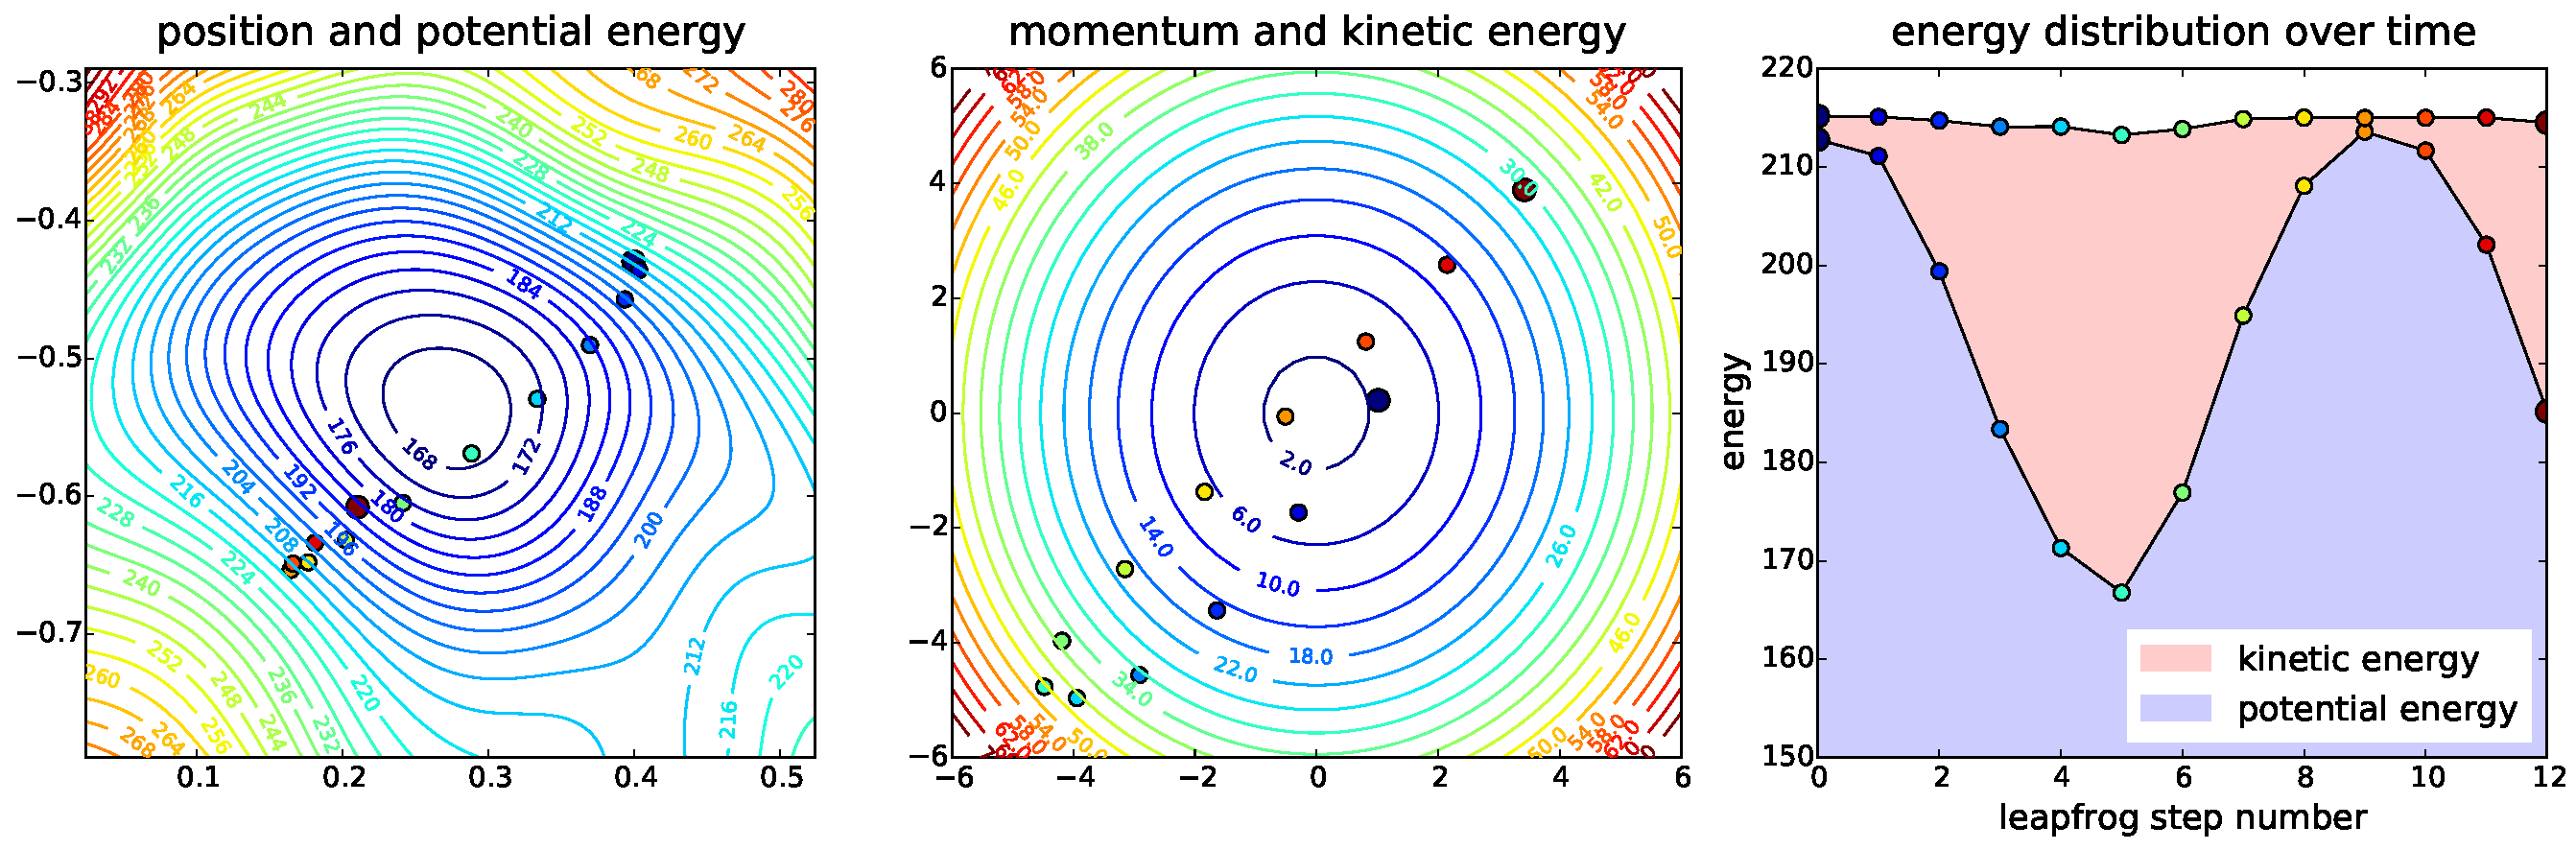
\includegraphics[width=2.05\columnwidth]{figures/hmc_motion_1hmc_12lf.pdf}
\caption{Dynamics of a particle under HD computed using the leapfrog method. Each computed point along the discretized trajectory is indicated by a separate color ranging from dark blue (starting point) to dark red (final point). The left plot shows the position of the particle with the prescribed potential energy represented by the contour plot. The centre plot depicts the momentum of the particle with the kinetic energy at each point indicated by the contours. In the plot on the right the energy distribution of the particle over time is given, with the potential energy in blue and the kinetic energy in red. Due to the discretization the total energy is not exactly conserved.}
\label{fig:HMC_MOTION_1hmc_12lf}
\end{figure*}

In such a physical system the kinetic energy is then given by $K(p) = p^T M^{-1} p /2$, where $M$ is called the mass matrix and in a physical context usually is $m I$, a scalar multiple of the identity. Here the scalar $m$ corresponds to the mass of the particle. With this kinetic energy we can retrieve Newton's equation of motion relating the acceleration $d^2q/dt^2$ to the force acting on a particle (given by $-\nabla U(q)$):
\begin{equation} \label{eq:NewtonsEquation}
\frac{d^2q}{dt^2} = M^{-1} \frac{dp}{dt} = - M^{-1} \frac{\partial H}{\partial q} = - M^{-1} \nabla U(q)
\end{equation}

The key advantage of HD over other formulations of classical dynamics is that analytic solutions to the above system have three crucial properties \parencite{Neal2011}:
\begin{itemize}
\item Reversibility: The mapping $T_s$ from the state $(q(t), p(t))$ at some time point $t$ to the state at $t+s$ ($s > 0$) is one-to-one and hence reversible. Thus by running time backwards, i.e.\ negating both time derivatives in Hamilton's equations, we can uniquely determine previous states.
\item Volume preservation: $T_s$ conserves volume in $(q, p)$-space, so applying it to some region of a certain volume results in a region of the same volume.
\item Conservation of the Hamiltonian: The Hamiltonian $H(q, p)$ is invariant with time, so $dH/dt = 0$.
\end{itemize}

All three of these properties would be useful in the application of the HMC algorithm, but due to the inevitable discretization of the differential equation not all of them can be preserved. The leapfrog method, which will be explained below, maintains reversibility and volume preservation and furthermore approximately conserves the Hamiltonian (see figure~\ref{fig:HMC_MOTION_1hmc_12lf}). This approximate conservation of the Hamiltonian makes it a so-called \textit{symplectic integrator}.

Given the step size $\epsilon$ the leapfrog method performs the following updates for $n \in \mathbb{N_0}$ starting from the initial state $(q^{(0)}, p^{(0)})$:
\begin{equation}
\begin{split}
p_i^{(n + 1/2)} &= p_i^{(n)} - \frac{\epsilon}{2} \frac{\partial U}{\partial q_i}(q^{(n)}) \\
q_i^{(n + 1)} &= q_i^{(n)} + \epsilon \frac{\partial K}{\partial p_i}(p^{(n + 1/2)}) \\
p_i^{(n + 1)} &= p_i^{(n + 1/2)} - \frac{\epsilon}{2} \frac{\partial U}{\partial q_i}(q^{(n + 1)})
\end{split}
\end{equation}
First a half-step for the momentum variables is computed, which is then used for a full position step. Finally, a second momentum half-step based on the updated position completes the leapfrog step. Since each of these updates is simply a shear transformation in $(q, p)$-space and therefore has a determinant of 1, a complete leapfrog step also has a determinant of 1 and is volume-conserving. If we perform multiple leapfrog steps, we can jump directly from $p_i^{(n + 1/2)}$ to $p_i^{(n + 3/2)}$ for greater efficiency.

With the usual choice for the kinetic energy $K(p) = p^T M^{-1} p /2$ and some manipulation of the above equations we can obtain an alternative formulation of the leapfrog method, which is more intuitive (but computationally more expensive):
\begin{equation}
\begin{split}
q^{(n + 1)} &= q^{(n)} + \epsilon M^{-1} p^{(n)}) + (\epsilon^2/2) M^{-1} F(q^{(n)}) \\
p^{(n + 1)} &= p^{(n)} + \epsilon (F(q^{(n)}) + F(q^{(n+1)}))/2,
\end{split}
\end{equation}
where $F(q) = - \nabla U(q)$ is the force acting on the particle at position $q$ due to the potential energy landscape. Since $M$ corresponds to the mass of the particle, $M^{-1} p$ gives its velocity and $M^{-1} F(q)$ its acceleration. From the first equation we see that the leapfrog method updates the position assuming motion under constant acceleration: $q(t) = q_0 + v_0 t + 1/2 a t^2$ with a initial position $q_0 = q^{(n)}$, initial velocity $v_0 = M^{-1} p^{(n)}$ and acceleration $a = M^{-1} F(q^{(n)})$. The second equation, which gives the momentum update, is simply a discretized version of the basic relationship $dp/dt = F$, i.e.\ force equals change of momentum, using the average of the forces at the start and the end point.

The local error of the leapfrog method, i.e.\ the error incurred in a single step, has order $\epsilon^3$; the global error, i.e.\ the error in the solution over a fixed time interval $L$, has order $\epsilon^2$. As a symplectic integrator the leapfrog method approximately conserves the Hamiltonian, so that the global error in the Hamiltonian, which is also order $\epsilon^2$, usually does not grow exponentially with the simulation length $L$ (with $\epsilon$ fixed) as it may for many other integration schemes \parencite{Neal2011}.

\subsection{The HMC algorithm}
\label{sec:HMCAlgorithmSection}
\subsubsection{Relating probability density to energy}
In order to apply HD within an MCMC method to sample from some target distribution, we need to derive appropriate energy functions. A key relationship in statistical mechanics is
\begin{equation}
P(s) = \frac{1}{Z} \exp \left(- \frac{E(s)}{T} \right),
\end{equation}
relating the probability density function $P(s)$ for observing a particle in state $s$ with the energy $E(s)$ of that state. Here, $T$ is the temperature of the system\footnote{$T$ is assumed here to be given in units such that the Boltzmann constant is 1.} and $Z$ is a normalization constant such that the total probability over all states equals 1. The distribution given by this probability density function is called the \textit{canonical distribution}.

By inverting this relationship we can derive the appropriate energy from any target distribution (w.l.o.g.\ setting $T=1$). The potential energy $U(q)$, whose canonical distribution has the target density $\tilde{P}(q)$, is thus given by $U(q) = -\log \left( \tilde{P}(q) \right) - \log Z$,
where we can drop the $\log Z$ term because energies only influence the particle motion through their derivatives. This also means that we do not need $\tilde{P}(q)$ to be normalized. A closer look at $U(q)$ reveals that it is the negative log-likelihood (NLL) of $\tilde{P}(q)$, which is frequently used as a minimization objective in machine learning. Therefore, this potential energy will promote motion towards low NLL points and thus the points proposed by motion simulation with this potential energy will tend to have a higher likelihood than those proposed by other methods.

For the simulation by HD the state of the system consists of the variable of interest $q$ plus an auxiliary momentum variable $p$ of the same size and so is given by the $2d$-dimensional $s = (q, p)$. With the potential energy $U(q)$ derived from the target distribution as described above, the Hamiltonian of this system is given by $H(q, p) = U(q) + K(p)$ for some kinetic energy $K(p)$ of our choice. Due to the additive nature of this Hamiltonian the joint canonical distribution of $(q, p)$ factorizes:
\begin{equation}
\begin{split}
p(q, p) &= \frac{1}{Z} \exp \left( -H(q, p) \right) \\
			&\propto \tilde{P}(q) \cdot \exp{(-K(p))}
\end{split}
\end{equation}

\subsubsection{Choice of kinetic energy}
In order to obtain a Markov chain, whose invariant distribution is the canonical distribution, some restrictions apply to the choice of kinetic energy \parencite{Betancourt2014}. In particular the corresponding canonical momentum distribution must have a mean of zero, since otherwise the resulting drift in the position variables makes convergence to the canonical distribution impossible. While it is possible to make the kinetic energy dependent on position in the Riemann Manifold Hamiltonian Monte Carlo method \parencite{Girolami2011}, this requires complicated modifications to the integrator and will not be considered here. \textcite{Betancourt2014} argue that there is little motivation to choose a kinetic energy other than the quadratic form from classical physics and in the following we will assume the usual choice for the kinetic energy
\begin{equation} \label{eq:KineticEnergy}
K(p) = p^T M^{-1} p/2
\end{equation}
for some positive definite mass matrix $M$. The corresponding canonical distribution (after normalization) $P_\textrm{kin}(p)$ is the multivariate Gaussian distribution with mean zero and covariance matrix $M$.

\subsubsection{The algorithm}
The HMC algorithm (see algorithm~\ref{alg:HMC}) produces the desired Markov chain \parencite{Neal2011}. There are two main steps in the algorithm: Firstly the simulation of HD using a reversible and volume-preserving integrator, e.g. the leapfrog method, and secondly a Metropolis-Hastings acceptance step to ensure the desired invariant distribution. Due to the momentum negation of the proposed state in the third step of the algorithm, the proposal distribution is symmetrical because of the reversibility of the integration method. As a result $\tilde{q}(\tilde{s}_t|s_{t-1}) = \tilde{q}(s_{t-1}|\tilde{s}_t)$ holds in the Metropolis-Hastings acceptance probability in equation~\eqref{eq:Metropolis-Hastings}, so the acceptance probability simplifies to
\begin{equation} \label{eq:AcceptanceProbability}
p_{\textrm{accept}}(s^*_{t-1}) = \min[1, \exp(-H(\tilde{s}_t) + H(s^*_{t-1}))].
\end{equation}

\begin{algorithm}
\caption{The HMC algorithm}\label{alg:HMC}
\begin{algorithmic}[1]
\Require Numeric integrator $HD(s)$ of Hamilton's equations simulating HD starting from state $s$ for a fixed length
\Require Current state $s_{t-1} = (q_{t-1}, p_{t-1})$
\State Sample new momentum $p^*_{t-1}$ from $P_\textrm{kin}$
\State Simulate HD starting from $s^*_{t-1} = (q_{t-1}, p^*_{t-1})$
\State Negate the momentum of the resulting state $s_\textrm{HD} = HD(s^*_{t-1})$ to obtain the proposed state $\tilde{s}_t = (q_\textrm{HD}, - p_\textrm{HD})$
\State Compute the acceptance probability $p_\textrm{accept}=p_\textrm{accept}(s^*_{t-1})$ as defined by equation~\eqref{eq:AcceptanceProbability}
\State Accept the move from $s^*_{t-1}$ to $\tilde{s}_t$ with probability $p_\textrm{accept}$
\State \textbf{Return} new state $s_t$
\end{algorithmic}
\end{algorithm}

It can be shown that this algorithm conserves the canonical distribution, which therefore also is the invariant distribution of the constructed Markov chain \parencite{Neal2011}. If the HD simulation was exact, then the Hamiltonian would be conserved, since negation of the momentum does not change the value of the Hamiltonian due to its symmetry. Therefore the acceptance probability would always be 1. However, numeric integrators cannot conserve the Hamiltonian exactly, necessitating the acceptance step. Still, for symplectic integrators, such as the leapfrog method, the numerical error usually remains bounded, allowing the rejection rate to be kept small even for long simulations.

\begin{figure*}[t]
\centering
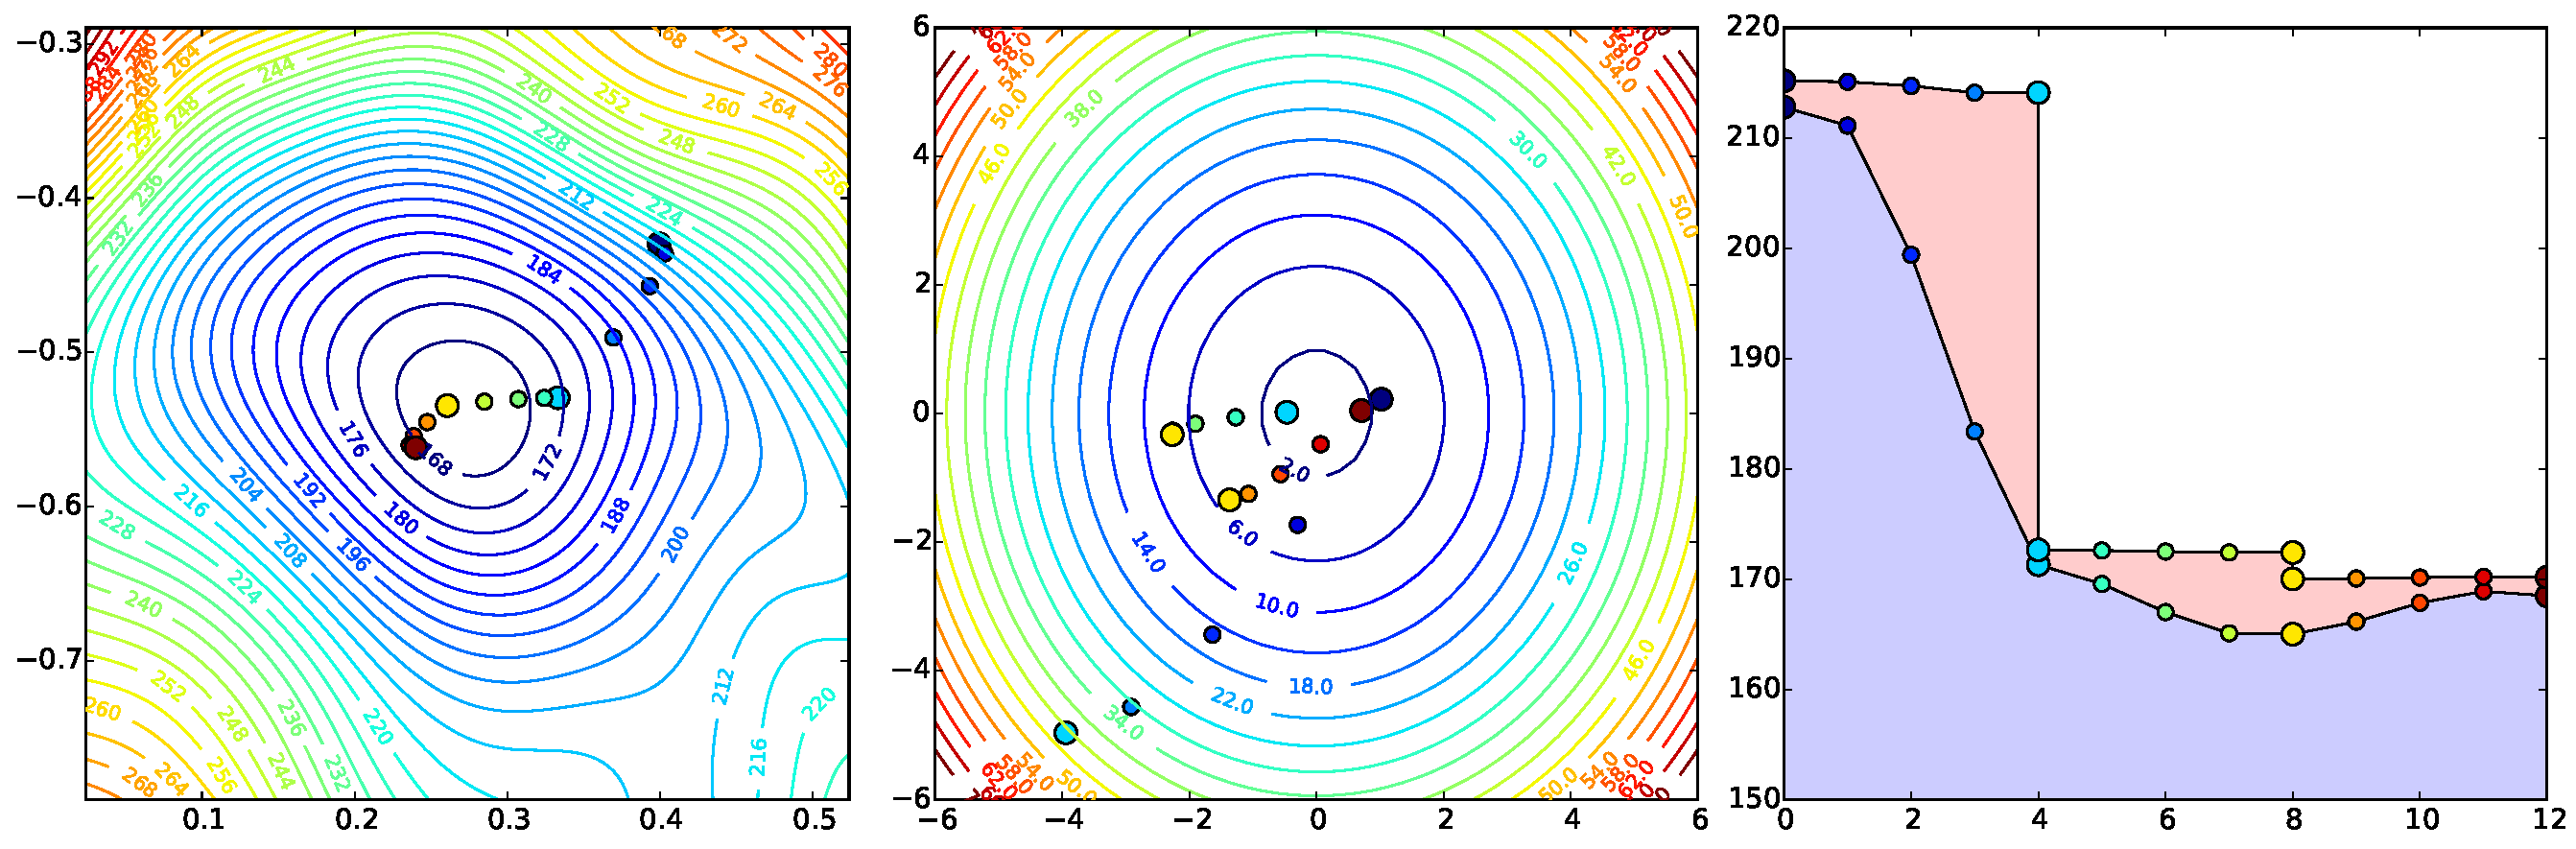
\includegraphics[width=2.05\columnwidth]{figures/hmc_motion_3hmc_04lf.pdf}
\caption{Evolution of a particle under the HMC algorithm with 3 HMC steps consisting of 4 leapfrog steps each. Each computed point along the trajectory is indicated by a separate color ranging from dark blue (starting point) to dark red (final point). Thicker dots highlight points, where momentum resampling was performed. The left plot shows the position of the particle with the prescribed potential energy represented by the contour plot. The centre plot depicts the momentum of the particle with the kinetic energy at each point indicated by the contours. Where the momentum was resampled, two identical dots are shown for the state before and after the resampling. In the plot on the right the energy distribution of the particle over time is given, with the potential energy in blue and the kinetic energy in red.}
\label{fig:HMC_MOTION_3hmc_04lf}
\end{figure*}

Due to the (approximate) conservation of the Hamiltonian during HD, the joint density $\exp \left( -H(q, p) \right)/Z$ of $(q,p)$ remains almost unchanged by steps 2 to 5 of the algorithm. Only the resampling of the momentum variable at the start of each HMC step allows large changes in the joint density. This can be seen in figure~\ref{fig:HMC_MOTION_3hmc_04lf}, where the evolution of a single particle is shown under the HMC algorithm. During the leapfrog steps the potential energy of the particle is partly converted to kinetic energy. With the newly drawn momentum the kinetic energy of the particle is smaller than before in this example leading to a decrease of its total energy. The sampled kinetic energy is given by $(1/2) p^T M^{-1} p$ (ignoring additive constants), which is $(1/2) \cdot \chi^2_d$-distributed for any $M$, if $p \sim P_\textrm{kin}(p)$. For the two-dimensional example in the figure this means that on average a particle gets a kinetic energy of 1 at the start of each HMC step, which could be converted into potential energy. Since the craters in the potential energy landscape are much deeper, particles are very unlikely to leave such a crater once they are caught inside.

Simulating an ensemble of particles illustrates how the convergence to the desired distribution happens in the HMC algorithm. In figure~\ref{fig:HMC_Effect_Illustration} particles were distributed according to some supposed distribution different from the desired distribution, which determines the energy landscape. After the first HMC step (bottom row of plots) the particles have mostly slid downhill, which can also be seen in the change in their potential energy (plots in the right column). Correspondingly, they have picked up kinetic energy, which will, however, be removed at the start of the next HMC step. In this way, the HMC steps initially reduce the amount of potential energy in the system corresponding to an increase of the likelihood of the particles w.r.t.\ the target distribution. By sampling a new momentum at the start of each HMC step, instead of for example setting it to 0 (in which case all the particles would gather at the low point of the potential energy), we ensure that the particles remain spread out and are eventually distributed according to the target distribution. 

\begin{figure*}[t]
\centering
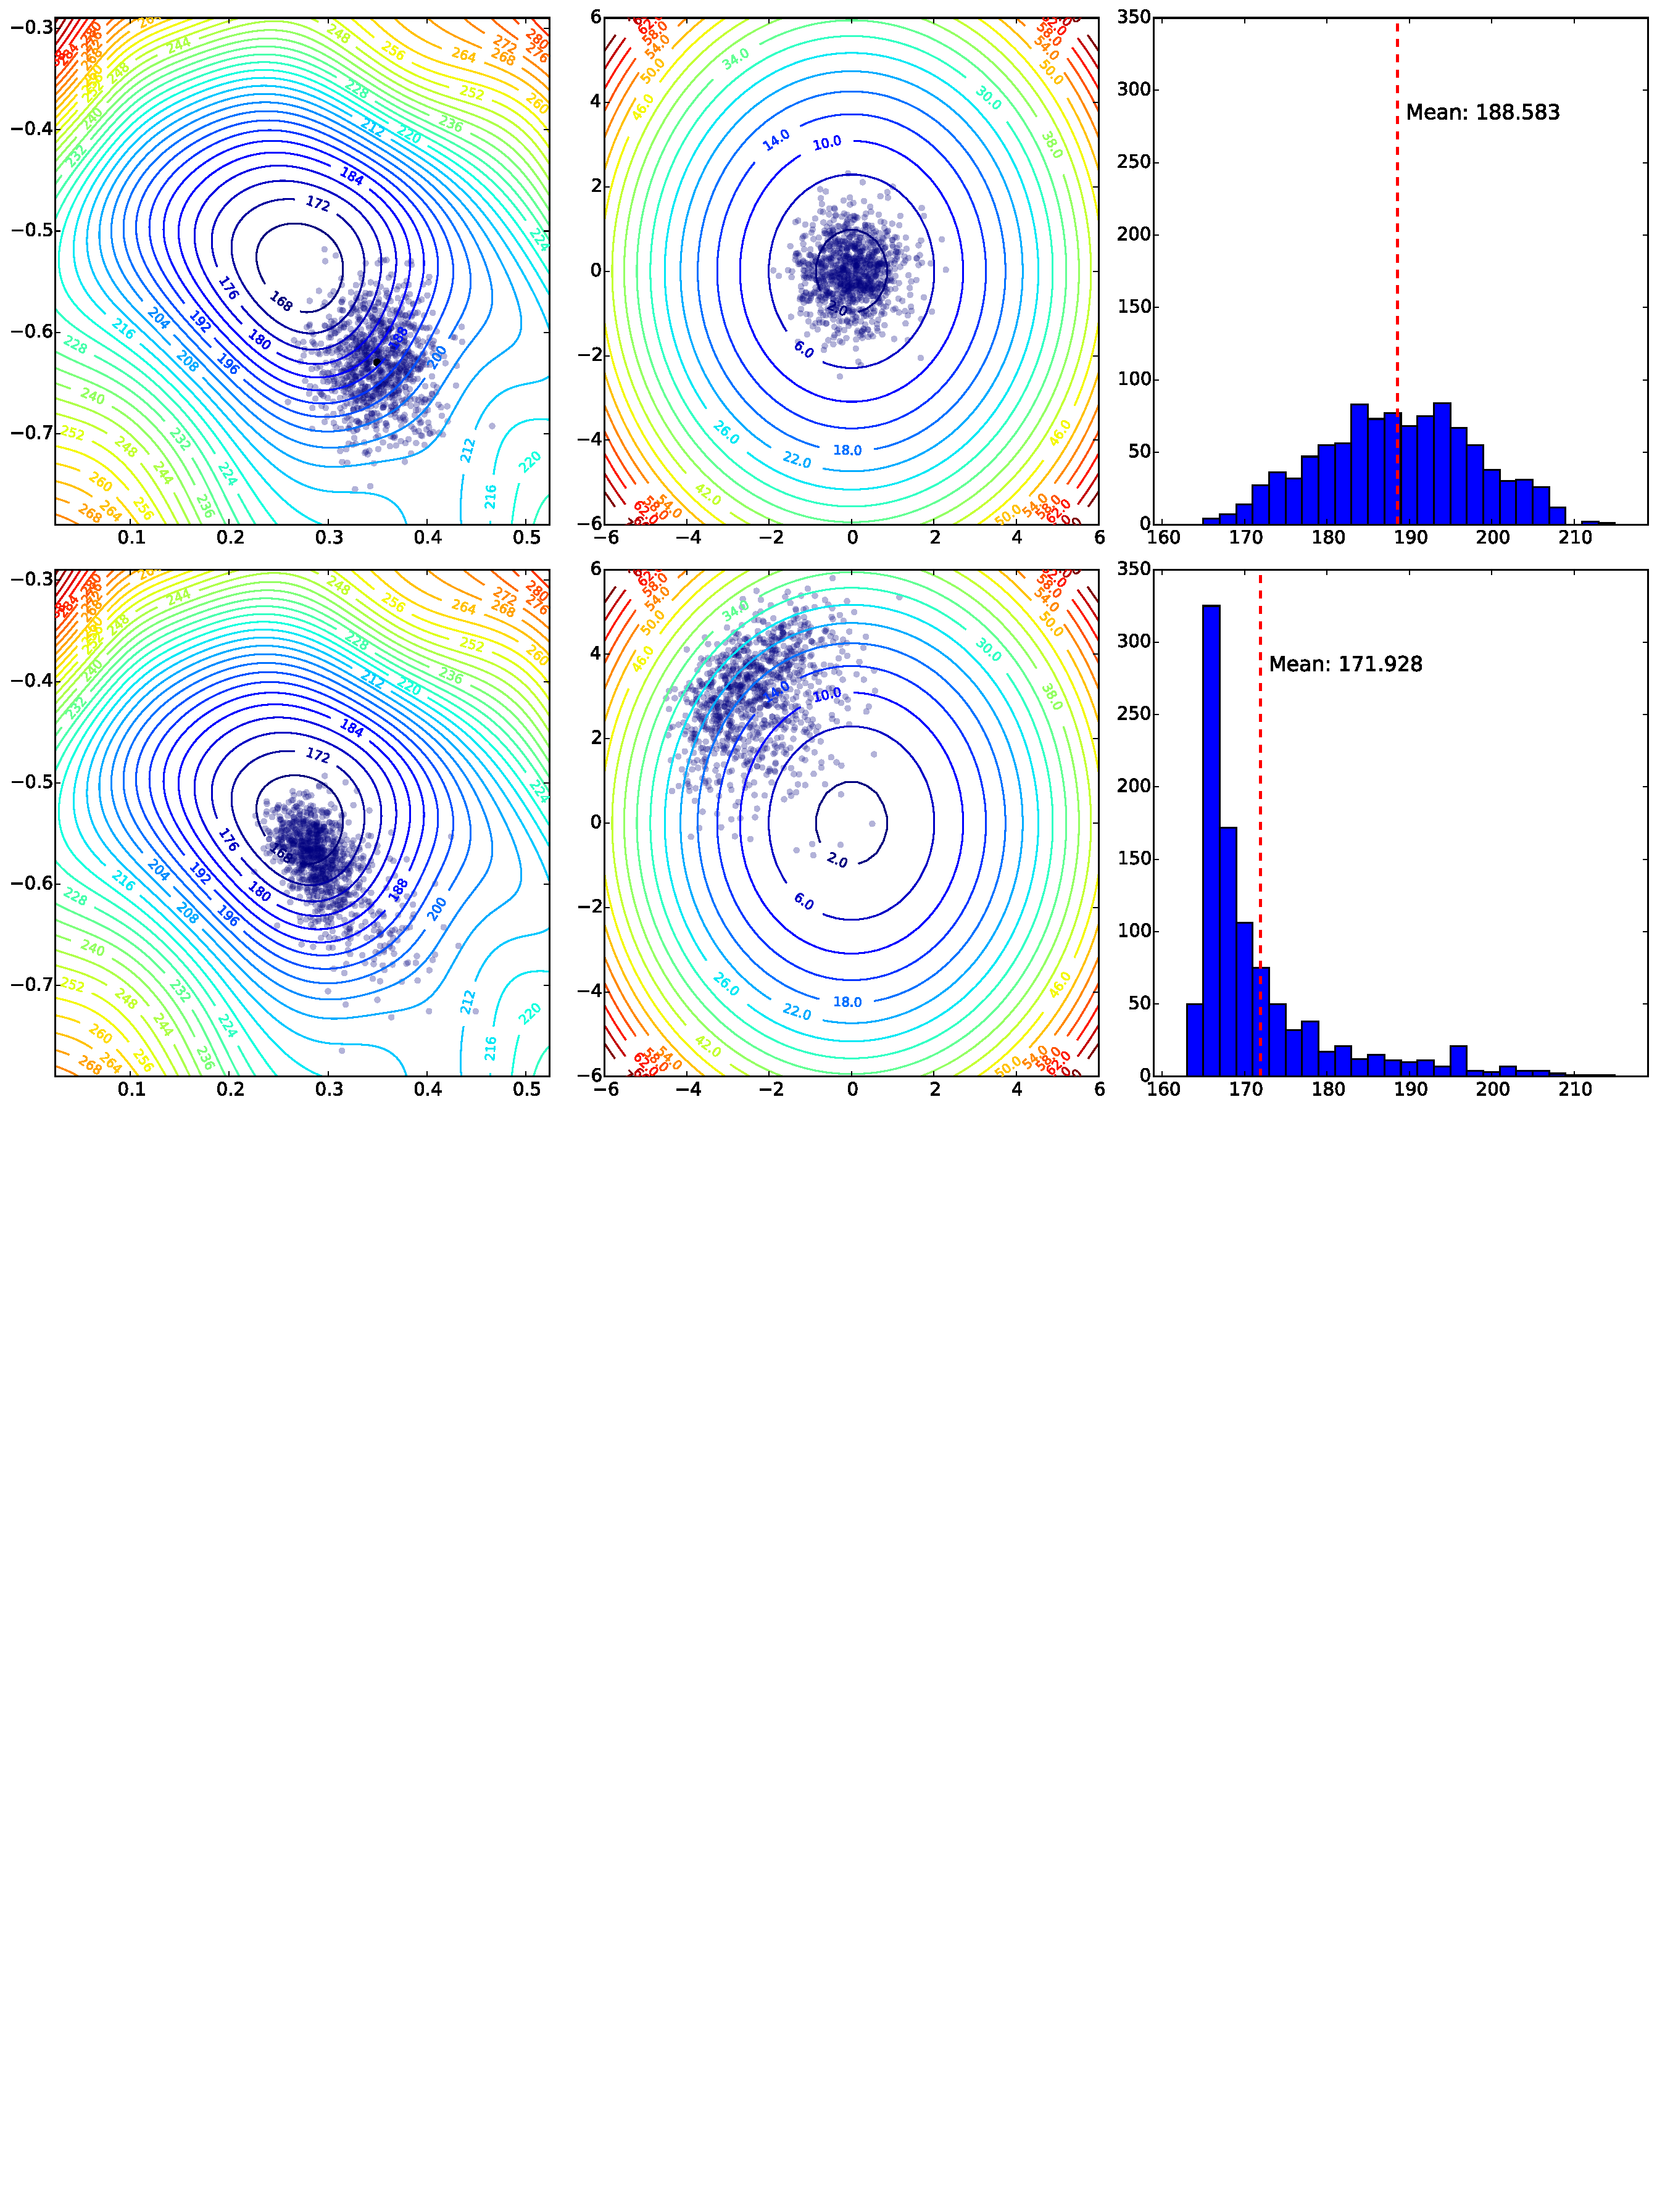
\includegraphics[width=2.05\columnwidth]{figures/hmcvi_distrib_example_top.pdf}
\caption{Evolution of an ensemble of 1000 particles under the HMC algorithm: The first row of plots shows the initial state of the system and the second row the state after an HMC step. The plots on the left give the positions of the particles with the prescribed potential energy represented by the contour plot. The centre plots depict the arrival momenta of the particles with the kinetic energy indicated by the contours. The right-hand plots show histograms of the potential energies of the particles.}
\label{fig:HMC_Effect_Illustration}
\end{figure*}

\subsection{Effect of the kinetic energy covariance matrix}
\label{sec:EffectOfKineticEnergyChoice}

For simplicity we restrict the kinetic energy (see eq.~\eqref{eq:KineticEnergy}) to be a positive-definite quadratic form, but not necessarily with a scalar multiple of the identity as mass matrix as the physical intuition of particle mass would suggest. A possible interpretation of such a "mass" matrix would be that the inertial mass of the particle, i.e.\ its resistance to change in velocity, is non-isotropic. In other words, the particle is more responsive to forces in some directions than in others. This somewhat non-physical freedom, however, has a very nice effect in the HMC algorithm: It allows an implicit rescaling of the $q$-space as explained below.

Such a rescaling can be very beneficial for the numerical solution, because the most restricted direction (with the most extreme changes in potential energy) limits the step length $\epsilon$ to be used in the discrete simulation. If a larger step length is used, the approximations of the energy surface used in the simulation are too coarse in the restricted direction and the discretization error becomes very large. As a result one may have to choose a very small step size, but this then limits the motion in the less restricted directions, where a larger step size would allow faster movement through the state space. Therefore, by rescaling the space we can achieve a more equal scaling in each direction, so that neither large errors nor slow exploration hamper the performance of the algorithm.

To see the connection between the mass matrix and the rescaling of $q$-space, assume the numerics of the dynamics w.r.t.\ the original variables $(q, p)$ were badly scaled when using the physically intuitive $K(p) = p^T p/2$ (taking $m=1$ for simplicity). Further suppose a transformation $q' = A^{-1} q$ with $p'=p$ and the same kinetic energy would yield a better scaling for some non-singular matrix $A$. Then the target distribution for $q'$ is given by $\tilde{P}'(q') = \tilde{P}(Aq')/|\det(A^{-1})|$ in terms of the original target distribution $\tilde{P}(q)$. Hence, the corresponding potential energy is $U'(q') = U(Aq')$, where we can drop the additive $\log(|\det(A^{-1})|)$ term. From Hamilton's equations (see equation~\eqref{eq:HamiltonsEquations}) for this system we get the following equations for the motion in terms of the original variables $(q, p)$:
\begin{equation}
\begin{split}
\frac{dq}{dt} &= A \frac{dq'}{dt} = Ap' = Ap \\
\frac{dp}{dt} &= \frac{dp'}{dt} = - \nabla U'(q') = - A^T \nabla U(q)
\end{split}
\end{equation}
The evolution of the position variable $q$ is thus given by (compare Newton's equation of motion~\eqref{eq:NewtonsEquation}):
\begin{equation} \label{eq:EvolutionQTransformed}
\frac{d^2q}{dt^2} = A \frac{dp}{dt} = - A A^T \nabla U(q)
\end{equation}

Now alternatively, let us consider the untransformed system, but with the kinetic energy $K''(p) = p^T A A^T p$. Then Hamilton's equation give us:
\begin{equation}
\begin{split}
\frac{dq}{dt} &= A A^T p \\
\frac{dp}{dt} &= - \nabla U(q),
\end{split}
\end{equation}
which results in the same evolution of the variable of interest $q$ as the direct transformation of $q$ above (compare equation~\eqref{eq:EvolutionQTransformed}). Regarding the evolution of $q$ these two approaches are thus identical (although the $p$ trajectories differ).

Introducing this transformation via the kinetic energy rather than transforming $q$ directly has the advantage, that we do not manipulate the variables of interest, which may be needed in their original form. Instead, we can achieve the same rescaling by modifying the auxiliary momentum variables, which do not have any external significance.

\subsection{Partial momentum update}
\label{sec:PartialMomentumUpdate}
If the number of leapfrog steps is small, subsequent points in the Markov chain generated by the HMC algorithm may be close to each other and highly correlated. This is especially obvious, if we imagine a flat plateau in the potential energy surface: Whatever momentum is sampled at the start of the HMC step, the simulated motion may frequently end at some other point still on the plateau, if the number of leapfrog steps is small. There the same may happen again, perhaps even bringing us back to the previous point, leading to an inefficient random-walk-like behaviour on this plateau.

To counter such a behaviour \textcite{Horowitz1991} proposed an extension to HMC, where the momentum is only partially updated. So instead of overwriting the momentum variable with a random sample from the canonical momentum distribution, the idea is to use a weighted sum of the current momentum and the newly drawn sample. By doing this the particle does not completely loose its current momentum after each HMC step, but continues in a similar direction as before. In the plateau example above, this means the particle is very unlikely to double back on its previous progress and will rather travel across the plateau in a directed fashion, avoiding the random-walk-like behaviour of the base HMC algorithm.

Some care must be taken in combining the current momentum $p_{t-1}$ with the new sample $p_\textrm{samp}$, because this momentum scrambling step must conserve the canonical distribution. This can be done by defining the updated momentum $p^*_{t-1}$ by
\begin{equation} \label{eq:partialMomentumUpdate}
p^*_{t-1} = \alpha \cdot p_{t-1} + \sqrt{1 - \alpha ^2} \cdot p_\textrm{sampled}
\end{equation}
for some $\alpha \in [-1, 1]$. In the converged chain both $p_{t-1}$ and $p_\textrm{sampled}$ are distributed according to the canonical distribution (Gaussian with mean zero and covariance matrix $M$), so $p^*_{t-1}$ will also be Gaussian and have mean zero. Since $p_{t-1}$ and $p_\textrm{sampled}$ are also independent of each other, the covariance is $\Cov(p^*_{t-1}) = \alpha^2 \cdot M + (1 - \alpha ^2) \cdot M = M$ as required.

\begin{algorithm}
\caption{The HMC algorithm with partial momentum updates}\label{alg:HMCWithPartial}
\begin{algorithmic}[1]
\Require Numeric integrator $HD(s)$ of Hamilton's equations simulating HD starting from state $s$ for a fixed length
\Require Current state $s_{t-1} = (q_{t-1}, p_{t-1})$
\State Sample new momentum $p_\textrm{samp}$ from $P_\textrm{kin}$
\State Update the momentum as in equation~\eqref{eq:partialMomentumUpdate} to obtain $p^*_{t-1}$
\State Simulate HD starting from $s^*_{t-1} = (q_{t-1}, p^*_{t-1})$
\State Negate the momentum of the resulting state $s_\textrm{HD} = HD(s^*_{t-1})$ to obtain the proposed state $\tilde{s}_t = (q_\textrm{HD}, - p_\textrm{HD})$
\State Compute the acceptance probability $p_\textrm{accept}=p_\textrm{accept}(s^*_{t-1})$ as defined by equation~\eqref{eq:AcceptanceProbability}
\State Accept the move from $s^*_{t-1}$ to $\tilde{s}_t$ with probability $p_\textrm{accept}$
\State Negate the momentum to obtain the new state $s_t$
\State \textbf{Return} new state $s_t$
\end{algorithmic}
\end{algorithm}

Algorithm~\ref{alg:HMCWithPartial} shows the steps in the improved version of the HMC algorithm for generating the next state of the Markov chain. Like the original HMC algorithm (algorithm~\ref{alg:HMC}), which can be recovered by setting $\alpha = 0$, this extension preserves the joint canonical distribution and thus yields a Markov chain with the required properties. Step 7, which is missing in the base version, is important for the case with partial momentum updates: If the proposed state was accepted, this step reverses the earlier momentum negation so that the particle keeps its direction. If the proposal was rejected, then it flips the momentum and the particle doubles back on itself. This can be clarified by combining steps 6 and 7:
\begin{equation} \label{eq:StateAfterAcceptReject}
s_t := \begin{cases} s_\textrm{HD} & \textrm{if accepted} \\ 
								(q_{t-1}, -p^*_{t-1}) & \textrm{if rejected}
					  \end{cases}
\end{equation}
For a better understanding, the order and used nomenclature of the states, which will be needed to derive the variational lower bound in section~\ref{sec:HMCVI}, are illustrated in figure~\ref{fig:HMC_schematic}.

\begin{figure}
\centering
\includegraphics{figures/hmc_illustration.tikz}
\caption{Flow chart illustrating the steps of the HMC algorithm with partial momentum updates.}
\label{fig:HMC_schematic}
\end{figure}

While the partial momentum update brings little benefit, if the number of leapfrog steps is large, it was reported to be beneficial for chains with shorter-than-optimal trajectories \parencite{Neal2011}. Because of computational limitations this will usually be the case in our application of HMC.
\section{VI with HMC}
\label{sec:HMCVI}
As suggested in \parencite{Salimans2014} HMC is a very good MCMC method to be used within MCVI as introduced in section~\ref{sec:MCVI}, because it is very efficient, usually requiring fewer steps than other methods for good convergence. However, some care must be taken in the derivation of the auxiliary lower bound, since now the state of the underlying MCMC chain is not just the variable of interest $z$ but also the auxiliary momentum variable, which we will call $v$ as it is related to velocity. So the complete state is the $2d$-dimensional $s=(z, v)$, corresponding to the state $(q, p)$ in the previous section, and the transition $(z_{t-1}, v_{t-1})$ to $(z_t, v_t)$ is obtained by the Hamiltonian Monte Carlo algorithm as described above. The appropriate potential energy $U(z)$ is derived from the posterior density $p(z|x) \propto p(x, z)$, which is known upto a multiplicative constant from Bayes' Theorem:
\begin{equation} \label{eq:VIwithHMCPotEnergy}
U(z) = -\log(p(x, z))
\end{equation}

Unless stated otherwise, the results below will hold for the more general algorithm with partial momentum update, from which the standard HMC algorithm can be recovered by setting $\alpha = 0$. For notational ease we will write $u_{t-1}$ for the updated momentum, which was referred to as $p^*_{t-1}$ in the previous section.

%TODO Graphik zur Reihenfolge/Bezeichnung der verschiedenen Zustände innerhalb eines HMC Schritts verlinken
\label{sec:KinEnergyMayDependOnX}
For the initial state of the chain we sample the position from a parametric approximation $q_0(z_0|x)$ as in Variational Inference and the momentum from the distribution $P_\textrm{kin}(v_0|x)$ corresponding to the chosen kinetic energy. Interestingly, there is no theoretical reason for the kinetic energy to be independent of $x$, which can be exploited to improve the quality of the bound (see section~\ref{sec:MassMatrixChoice} below).

\subsection{Deriving the variational lower bound}

The auxiliary lower bound given in equation~\eqref{eq:MCVIAuxLowerBound} derived for the base case can not be used with HMC, since the transition density $q(z_t|z_{t-1}, x)$ is intractable when using the HMC algorithm. The transition densities $q(s_t|s_{t-1}, x)$, however, are nicely tractable, as will be shown below. To incorporate these the derivation of the auxiliary lower bound must be modified:\begin{equation}
\begin{split}
\log & p(x) \geq \mathcal{L} \\
& \geq \mathcal{L} - \E_{q(z_T|x)} \big[ D_{KL}[q(y | z_T, x) || r(y | z_T, x)] \big] \\
& = \E_{q(y, z_T|x)} \Big[ \log p(x, z_T) - \log q(y, z_T|x) \\
& 	\qquad\qquad\qquad\qquad 							+ \log r(y | z_T, x) \Big] \eqqcolon \mathcal{L}_{\textrm{aux}},
\end{split}
\end{equation}
where $y = (s_0, \dots, s_{T-1}, v_T)$.

Here the density of the forward chain can be decomposed using the Markov property into the tractable transition densities:
$\log q(y, z_T|x) = \log q_0(s_0|x) + \sum_{t=1}^T \log q(s_t|s_{t-1}, x)$, where for the initial state we use the density $q_0(s_0|x) = q_0(z_0|x) \cdot P_\textrm{kin}(v_0|x)$, from which it was also sampled.

For the auxiliary reverse density first note that we can rewrite $r(y | z_T, x) = r(s_0, \ldots, s_{T-1}| s_T, x) \cdot r_{\textrm{final}}(v_T | z_T, x)$ for some distribution $r_{\textrm{final}}(v_T|z_T, x)$, which approximates the final distribution of the velocity $v_T$ given the position $z_T$. By then assuming a Markov structure on the reverse model (as for the base case) we get
$\log r(y | z_T, x) = \log r_{\textrm{final}}(v_T | z_T, x) + \sum_{t=1}^T \log r(s_{t-1}|s_t, t, x)$,
where it is crucial to note that the reverse model $r$ may depend on the time step (as discussed in section~\ref{sec:MCVI}).

With these simplification we can rewrite the lower bound as
\begin{equation} \label{eq:HMCVIAuxLowerBound}
\begin{split}
&\mathcal{L_\textrm{aux}} = \E_{q(s_0, \ldots, s_T|x)} \Big[ \log p(x, z_T) - \log q_0(z_0|x) \\
&\;+ \log r_{\textrm{final}}(v_T | z_T, x) - \log P_\textrm{kin}(v_0|x)  \\ 
&\;+ \sum \limits_{t=1}^T \big( \log r(s_{t-1}|s_t, t, x) - \log q(s_t|s_{t-1}, x) \big) \Big],
\end{split}
\end{equation}
where auxiliary models must be learnt for the reverse transitions, i.e. for the reverse model $r(s_{t-1}|s_t, t, x)$, and for $r_{\textrm{final}}(v_T | z_T, x)$, which predicts the final momentum given the final position. We will refer to this model as the final momentum model. Additionally we can learn the step size $\epsilon$ and the covariance matrix (or mass matrix) $M$ of the kinetic energy used by the HMC algorithm. The number of HMC steps and the number of leapfrog steps per iteration have to be integer and are therefore complicated to learn. For this reason they will be considered as hyper parameters of the algorithm, which are fixed in advance. Optimization of this bound is done as for MCVI (compare section~\ref{sec:MCVI}) by using Monte Carlo estimates of the expectation of the gradient. For future reference let's call the optimization of this lower bound Hamiltonian Monte Carlo Variational Inference (HMCVI).

To evaluate this lower bound we need to compute the transition probabilities $q(s_t|s_{t-1}, x)$ implied by the HMC algorithm. A key observation here is that performing Hamiltonian Dynamics (HD) on the variables with a volume-preserving integrator, such as the leapfrog method, is a bijective and volume-preserving step. Therefore the change of variables between the proposed state $(\tilde{z_t}, \tilde{v_t})$ and the state $(z_{t-1}, u_{t-1})$, from which the HD simulation was started, is bijective and has a Jacobian determinant equal to 1. In the following we will write $HD(s)$ to mean the state obtained by applying HD to the state $s$, so $(\tilde{z}_t, \tilde{v}_t) = HD(z_{t-1}, u_{t-1})$. Similarly $revHD(s)$ will denote the state, which results from running HD backwards in time starting from $s$. Further $\delta[.]$ will be used to signify the Dirac delta function.

\subsection{Transition densities without the acceptance step}
\label{sec:TransitionDensitiesNoAcceptance}
Skipping the acceptance step in the HMC algorithm means that the proposed state is always accepted as the new state, so $(z_t, v_t) = (\tilde{z}_t, \tilde{v}_t)$. In this case the transition densities of the forward model follow directly from the bijectivity and volume-preservation of HD:
\begin{equation} \label{eq:ForwardTransitionNoAcceptance}
\begin{split}
q(s_t|&s_{t-1}, x) = q(z_t, v_t| z_{t-1}, v_{t-1}, x) \\
&= q'(revHD(z_t, v_t)|z_{t-1}, v_{t-1}, x) \\
&= q'(z^*_{t-1}, u_{t-1} |z_{t-1}, v_{t-1}, x) \\
&= q_U(u_{t-1}|v_{t-1}, x) \cdot \delta[{z^*}_{t-1} - z_{t-1}],
\end{split}
\end{equation}
where $(z^*_{t-1}, u_{t-1}) \coloneqq revHD(z_t, v_t)$. With $v_{\textrm{samp}} \coloneqq (u_{t-1} - \alpha \cdot v_{t-1})/{\sqrt{1 - \alpha^2}}$, the momentum drawn from the canonical momentum distribution in this step, we can further simplify
\begin{equation} \label{eq:qUDefinition}
q_U(u_{t-1}|v_{t-1}, x) = P_\textrm{kin}(v_{\textrm{samp}}|x) \cdot (\frac{1}{\sqrt{1 - \alpha^2}})^{d}
\end{equation}

For the reverse model $r(s_{t-1}|s_t, t, x)$ we can also exploit the properties of HD to simplify the model to be learnt (with the same notation):
\begin{equation} \label{eq:ReverseTransitionNoAcceptance}
\begin{split}
r(&s_{t-1}|s_{t}, t, x) = r(z_{t-1}, v_{t-1}| z_t, v_t, t, x) \\
&\;= r'(z_{t-1}, v_{t-1} |z^*_{t-1}, u_{t-1},t , x) \\
&\;= r_V(v_{t-1}|z_{t-1}, u_{t-1}, t, x) \cdot \delta[z^*_{t-1} - z_{t-1}] \\
\end{split}
\end{equation}
So the auxiliary reverse model is fixed except for the distribution $r_V$ of the arrival momentum $v_{t-1}$, with which the position $z_{t-1}$ was reached. To model this distribution we may use the position $z_{t-1}$, $x$ and the current time step $t$, as well as the updated momentum $u_{t-1}$, which was used in the step away from this point. If we assume a bias due to the initial state, all of these may contain information about the arrival momentum, so they all should be included for a better fitting model.

For the computation of the lower bound the Dirac functions are problematic because their value is infinite, when their argument equals $0$. However, since a delta function appears both in the forward and in the reverse model (whose log-likelihoods are subtracted from each other), the Dirac functions can be handled: The Dirac function $\delta(x)$ can be approximated by a function with a small but extended support, say of width $\kappa$, where its value is $1/\kappa \cdot \mathbb{I}\big[x \in (x - 0.5 \cdot \kappa, x + 0.5 \cdot \kappa)\big]$, so that the property of the Dirac function of integrating to 1 is preserved. Here $\mathbb{I}[x \in A]$ denotes the indicator function of some set $A$, which equals $1$ if $x \in A$ and $0$ otherwise. Taking the limit of this for $\kappa \rightarrow 0$ returns the Dirac function. By subtracting the logarithms of two Dirac functions their height factor, i.e. $1/\kappa$, cancels, so we can safely take the limit and are left with two indicator functions instead of the two Dirac functions.

When computing the lower bound we only require the transition densities of the points generated by the algorithm and these are generated from the previous points by HD. Therefore for all of these transitions the indicator functions will take the value $1$, so taking the logarithm of these terms does not lead to any problems.

The main drawback of leaving out the acceptance step is that the canonical distribution of the state is no longer preserved by the Markov chain transitions and as a result the chain does no longer converge to the canonical distribution. This means that samples from the converged chain will not follow the target distribution. While this would rule out this version of the HMC algorithm for its usual sampling application, it may still be of use for our improved approximation of the posterior distribution, where it is usually only feasible to perform a very limited number of HMC steps for computational reasons. For this reason loosing the asymptotic convergence is acceptable, since the new invariant distribution should differ only slightly from the target distribution and this difference should have little effect on the start of the chain. Apart from the computational simplifications leaving out the acceptance step also makes the algorithm less wasteful, since no proposals are thrown away.

\subsection{Transition densities with the acceptance step}

A drawback of the basic MCVI approach is that when using the latent variable $z$ as the state and proposal density $\tilde{q}(z_t|z_{t-1}, x)$ for new points, then we cannot include the acceptance step of the Metropolis-Hastings algorithm \parencite{Salimans2014}: Letting $\rho(z_{t-1}, z_t)$ be the probability of accepting the transition from $z_{t-1}$ to $z_t$, the transition density is given by $q(z_t|z_{t-1}, x) = \tilde{q}(z_t|z_{t-1}, x) \cdot \rho(z_{t-1}, z_t) + \delta[z_t - z_{t-1}] \cdot P_\textrm{reject}(z_{t-1})$, where $P_\textrm{reject}(z_{t-1}) = \int_{\tilde{z}_{t}} \tilde{q}(\tilde{z}_t|z_{t-1}, x) \cdot (1 - \rho(z_{t-1}, \tilde{z}_t)) d\tilde{z}_t$ is usually intractable. A possible solution would be to explicitly include a binary random variable in the state, which records the acceptance of the previous step. However, this would lead to non-differentiability of the lower bound.

Exploiting the structure of HMC we can bypass this problem and include the acceptance step without introducing any new variables, because in case of rejection the momentum variable is not reset to its previous value, but keeps the updated value (see equation~\eqref{eq:StateAfterAcceptReject} in section~\ref{sec:PartialMomentumUpdate}). In this way it stores the proposed state, which was rejected, making the transition density tractable as shown below.

Crucially by including the acceptance step in the algorithm convergence of the approximation of the posterior to the true posterior is guaranteed, so by performing a sufficient number of HMC steps the obtained approximation can be made to fit arbitrarily well.

\subsubsection{Forward model}

For the derivation of the transition density $q(s_t|s_{t-1}, x)$ let $A$ be the random variable indicating, whether the proposed move was accepted or not, i.e. $A=1$, if the move was accepted, and $A=0$ otherwise. For extra clarity we will in the following write out the probability density functions (denoted by $f$) with the variables explicitly given in the subscript, so for example $q(s_t|s_{t-1}, x) = f_{S_t|S_{t-1}, X}(s_t|s_{t-1}, x)$. Then using the law of total probability we can decompose this as:
\begin{equation}
\begin{split}
f_{S_t|S_{t-1}, X}&(s_t|s_{t-1}, x)= \sum_{a=0}^1 \int \limits_{u_{t-1}} f_{S_t, A, U_{t-1}|S_{t-1}, X}(s_t, a, u_{t-1}|s_{t-1}, x) du_{t-1} \\
& = \sum_{a=0}^1 \int \limits_{u_{t-1}} f_{S_t|A, U_{t-1}, S_{t-1}, X}(s_t| a, u_{t-1}, s_{t-1}, x) \\
& \qquad\cdot \mathbb{P}(A = a|U_{t-1} = u_{t-1}, S_{t-1} = s_{t-1}, x) \cdot f_{U_{t-1}|S_{t-1}, X}(u_{t-1}|s_{t-1}, x) du_{t-1}
\end{split}
\end{equation}
Each term in this expression can be computed:
\begin{itemize}
\item $f_{U_{t-1}|S_{t-1}, X}(u_{t-1}|s_{t-1}, x) = q_U(u_{t-1}|v_{t-1}, x) = P_\textrm{kin}(v_{\textrm{samp}}|x) \cdot (\frac{1}{\sqrt{1 - \alpha^2}})^{d}$ as in equation~\eqref{eq:qUDefinition} for the forward transition without the acceptance step.
\item $\mathbb{P}(A=1|S_{t-1} = s_{t-1}, U_{t-1} = u_{t-1}, x) = p_{\textrm{accept}}(z_{t-1}, u_{t-1})$ as in equation~\eqref{eq:AcceptanceProbability}
\item $\mathbb{P}(A=0|S_{t-1} = s_{t-1}, U_{t-1} = u_{t-1}, x) = 1- p_{\textrm{accept}}(z_{t-1}, u_{t-1})$
\item $f_{S_t|A, U_{t-1}, S_{t-1}, X}\big((z_t, v_t)| 1, u_{t-1}, s_{t-1}, x\big) = \delta \left[(z_t, v_t) - HD(z_{t-1}, u_{t-1}) \right]$
\item $f_{S_t|A, U_{t-1}, S_{t-1}, X}\big((z_t, v_t)| 0, u_{t-1}, s_{t-1}, x\big) = \delta \left[(z_t, v_t) - (z_{t-1}, -u_{t-1}) \right]$
\end{itemize}

Putting all of these together and integrating out the delta functions gives
\begin{equation}
\begin{split}
q(s_t |s_{t-1}, x) &= \delta \left[z_{\textrm{revHD}} - z_{t-1} \right] \cdot p_{\textrm{accept}}(z_{t-1}, v_{revHD}) \cdot q_U(v_{revHD}|v_{t-1}, x) \\
&\quad + \delta \left[ z_t - z_{t-1} \right] \cdot (1 - p_{\textrm{accept}}(z_{t-1}, -v_t)) \cdot q_U(-v_t|v_{t-1}, x)
\end{split}
\end{equation}
where we write $z_{\textrm{revHD}}$ and $v_{\textrm{revHD}}$ for the projections of $revHD(z_t, v_t)$ into $z$- and $v$-space respectively.

As we will see below, the reverse model densities will also contain a $d$-dimensional Dirac function in each summand, so we can apply the trick introduced in section~\ref{sec:TransitionDensitiesNoAcceptance} to replace Dirac functions by indicator functions. Here the indicator functions can be taken to indicate, whether the proposed state was accepted (in the first summand) and rejected (in the second), because the probability of exactly achieving the equality inside the $\delta$-function in the other case is negligible, i.e. if the move is accepted $z_t = z_{t-1}$ will not occur in practice. In the following we will write $\mathbb{I}_\textrm{accepted}$ for this indicator.

So we can regard each summand as treating one of the acceptance/rejection cases and since in the first summand $u_{t-1} = v_{revHD}$ and in the second summand $u_{t-1} = -v_t$, the term for the velocity in both cases becomes $q_U(u_{t-1}|v_{t-1}, x)$, where $u_{t-1}$ is the updated velocity generated in the algorithm outlined above. Also the $p_\textrm{accept}$ term is always computed from this $u_{t-1}$ and the current position $z_{t-1}$, so the transition density can easily be calculated during the sampling process as
\begin{equation}
q(s_t|s_{t-1}, x) = q_U(u_{t-1}|v_{t-1}, x) \cdot \Big( \mathbb{I}_\textrm{accepted} \cdot p_{\textrm{accept}} + (1 - \mathbb{I}_\textrm{accepted}) \cdot (1- p_{\textrm{accept}}) \Big),
\end{equation}
where we can also simplify $q_U(u_{t-1}|v_{t-1}, x)$ as in equation~\eqref{eq:qUDefinition}.

\subsubsection{Reverse Model}
\label{sec:TransDensitiesWithAcceptReverse}
In the lower bound approximation we also need a density approximation for moves backwards through the chain, i.e. for $r(s_{t-1}|s_t, t, x) = f_{S_{t-1}|S_t,T, X}(s_{t-1} | s_t, t, x)$. By again letting $A$ be the event of accepting the move from $S_{t-1}$ to $S_t$ we can apply the law of total probability to simplify the problem:
\begin{equation}
\begin{split}
f_{S_{t-1}|S_t, T, X}(s_{t-1} | s_t, t, x) &= \sum_{a=0}^1 f_{S_{t-1}, A|S_t, T, X}(s_{t-1}, a | s_t, t, x) \\
&= \sum_{a=0}^1 f_{S_{t-1} |A, S_t, T, X}(s_{t-1} | a, s_t, t, x) \cdot \mathbb{P}(A = a | S_{t} = s_{t}, t, x)
\end{split}
\end{equation}
The individual terms are now easier to handle:
\begin{itemize}
\item If we know that the previous move was accepted, we can use the reversibility of Hamiltonian Dynamics to obtain the state $S_{t-1}^* = (Z_{t-1}, U_{t-1})$, from which the HD-simulation was started, so
\begin{equation}
\begin{split}
f_{S_{t-1} |A, S_t, T, X}(s_{t-1} | 1, s_t, t, x) \\
&= f_{S_{t-1} |S_{t-1}^*, T, X}\big(s_{t-1} | revHD(s_t), t, x\big) \\
&= \delta \left[z_{t-1} - z_{\textrm{revHD}} \right] \cdot r_V(v_{t-1}|z_{\textrm{revHD}}, v_{\textrm{revHD}}, t, x) \\
&= \mathbb{I}_\textrm{accepted} \cdot r_V(v_{t-1}|z_{t-1}, u_{t-1}, t, x) 
\end{split}
\end{equation}
with $r_V$ as in equation~\eqref{eq:ReverseTransitionNoAcceptance} and the updated momentum $u_{t-1} = v_{\textrm{revHD}}$. As described earlier the $\delta$-function in the derivation is replaced by an indicator function by cancelling it against the $\delta$-function in the forward density.
\item If the previous move was not accepted, we know that the current state equals the state $S_{t-1}^*$ (with the velocity negated) from which the HD-transition was started, but rejected, so
\begin{equation}
\begin{split}
f_{S_{t-1} |A, S_t, T, X}(s_{t-1} | 0, s_t, t, x) &= f_{S_{t-1} |S_{t-1}^*, T, X}\big(s_{t-1} | (z_t, -v_t), t, x\big) \\
&= \delta \left[z_{t-1} - z_{t} \right] \cdot r_V(v_{t-1}|z_{t-1}, -v_t, t, x) \\
&= (1 - \mathbb{I}_\textrm{accepted}) \cdot r_V(v_{t-1}| z_{t-1}, u_{t-1}, t, x)
\end{split}
\end{equation}
where now $u_{t-1} = -v_t$ and the $\delta$-function is again converted to an indicator function by cancellation.

If these densities are computed during the sampling process, $u_{t-1}$ is actually known in both cases, since we generate it in the forward model and by the bijectivity of HD it is uniquely determined: If $\mathbb{I}_\textrm{accepted} = 1$, then $v_{\textrm{revHD}}$ is the updated velocity $u_{t-1}$ in the algorithm, and if $\mathbb{I}_\textrm{accepted} = 0$, then $-v_t$ is the updated velocity.
\item The probability $\mathbb{P}(A = 1|S_t = s_t, t, x)$ of accepting the previous step given the current position can be related to the distribution of $S_{t-1}^*$ by considering
\begin{subequations}
\begin{equation}
\mathbb{P}(A = 1|S_t = s_t, t, x) = \frac{f_{A, S_t|T, X}(1, s_t| t, x)}{f_{A, S_t|T, X}(1, s_t| t, x) + f_{A, S_t|T, X}(0, s_t| t, x)},
\end{equation}
where we can rewrite the terms using $p_\textrm{accept}(s)$ defined in equation~\eqref{eq:AcceptanceProbability}:
\begin{align}
\begin{split}
f_{A, S_t|T, X}(1, s_t| t, x) &= f_{A, S_{t-1}^*|T, X}\big(1, revHD(s_t)| t, x\big) \\
&= \mathbb{P}\big(A = 1| S^*_{t-1} = revHD(s_t), x\big) \cdot f_{S^*_{t-1}|T, X}\big(revHD(s_t)| t, x\big) \\
&= p_\textrm{accept}(revHD(s_t)) \cdot f_{S^*_{t-1}|T, X}\big(revHD(s_t)| t, x\big)
\end{split} \\
\begin{split}
f_{A, S_t|T, X}(0, s_t| t, x) &= f_{A, S_{t-1}^*|T, X}\big(0, (z_t, -v_t)| t, x\big) \\
&= \mathbb{P}\big(A = 0| S^*_{t-1} = (z_t, -v_t), x\big) \cdot f_{S^*_{t-1}|T, X}\big((z_t, -v_t)| t, x\big) \\
&= \big(1 - p_\textrm{accept}(z_t, -v_t)\big) \cdot f_{S^*_{t-1}|T, X}\big((z_t, -v_t)| t, x\big)
\end{split}
\end{align}
\end{subequations}
Now $p_\textrm{accept}(z_t, -v_t) = \min[1, \exp(-H(HD(z_t, -v_t)) + H(z_t, -v_t)]$, where $H(s)$ is the Hamiltonian of state $s$. So if the exponent of the second term is positive, then $p_\textrm{accept}(z_t, -v_t) = 1$ and inserting this in the above gives that $\mathbb{P}(A = 1|S_t = s_t, t, x) = 1$, so the move to $s_t$ must have been accepted.

If this is not the case then the above expression cannot be simplified further without reducing the flexibility of the model. So in this case one would ideally learn an approximation for $\mathbb{P}(A=1|S_t = s_t, t, x)$, taking $s_t$, $x$ and the time point $t$ as inputs, in effect trying to predict whether the previous move was accepted based on the current position. A good starting point for this model can be obtained by assuming that the Markov chain has already converged, in which case $S_{t-1}^*$ would follow the canonical distribution, so we would have $f_{S^*_{t-1}|T, X}(s| t, x) \propto \exp(-H(s))$. Inserting this in the above equations and noting, that $HD(z_t, -v_t) = revHD(z_t, v_t)$ by the invertibility of HD and $H(z_t, -v_t) = H(z_t, v_t)$ by symmetry of the kinetic energy, yields
\begin{equation}
\mathbb{P}(A = 1|S_t = s_t, t, x) = \exp(-H(revHD(s_t)) + H(s_t))
\end{equation}
So if $H(revHD(s_t)) \leq H(s_t)$, the previous move was always accepted. Otherwise, the probability needs to be learnt, but will tend towards $\exp(-H(revHD(s_t)) + H(s_t))$ as the chain converges. 
\item $\mathbb{P}(A = 0|S_t = s_t, t, x) = 1 - \mathbb{P}(A = 1|S_t = s_t, t, x)$
\end{itemize}

So a full auxiliary reverse model to capture the density of the backward Markov chain consists of two parts: Firstly the density estimating model for $r_V(v_{t-1}|z_{t-1}, u_{t-1}, t, x)$ as for the case without the acceptance step and secondly a model for $\mathbb{P}(A = 1|S_t = s_t, t, x)$. Regarding $r_V$ a small difference to the case without the acceptance step is, that here $v_{t-1}$ is not always the end of a previous HD simulation, but can also be equal to  $-u_{t-2}$, the updated momentum at the start of the previous simulation, if the resulting proposal was rejected. 

Putting these terms together the reverse transition density is given by
\begin{equation}
\begin{split}
r(s_{t-1} &| s_t, t, x) = r_V(v_{t-1}| z_{t-1}, u_{t-1}, t, x) \\
&\cdot \Big( \mathbb{I}_\textrm{accepted} \cdot \mathbb{P}(A = 1 | s_{t}, t, x) + (1 - \mathbb{I}_\textrm{accepted}) \cdot \mathbb{P}(A = 0 | s_{t}, t, x) \Big)
\end{split}
\end{equation}
With this last component for the computation of the auxiliary lower bound using the full HMC algorithm including the acceptance step we are now able to apply the full HMC algorithm within the MCVI framework. In particular, we recover the guaranteed convergence to the exact posterior, which was lost by skipping the acceptance step.

\subsection{Learning the mass matrix}
\label{sec:MassMatrixChoice}
In its usual application as a sampling algorithm the freedom in the configuration of the HMC is often a curse, since a lot of parameters have to be specified, for example the mass matrix and the step size. These choices may then dramatically change the performance of the algorithm. In our application, however, we can side-step this issue by allowing all continuous parameters of the algorithm to be learnt, in particular the mass matrix $M$. As explained in section~\ref{sec:EffectOfKineticEnergyChoice} choice of mass matrix is equivalent to a rescaling of the "position"-space (here the $z$-space), which may improve the convergence of the algorithm. It is important to keep in mind, that the space is not actually transformed, but that the mass matrix makes the algorithm behave as if the space was transformed.

In addition to this indirect contribution to the lower bound through improved convergence, the mass matrix also directly appears in the lower bound as the covariance matrix of the canonical momentum distribution: From the lower bound and the transition densities derived in the previous sections we see that for each HMC step a term $-\log P_\textrm{kin}(v_\textrm{samp}|x)$ appears. Here $P_\textrm{kin}$ is the density of the canonical momentum distribution, a zero-mean multivariate normal distribution with covariance matrix $M$, and $v_\textrm{samp}$ is a sample from this distribution. In the lower bound the expectation of this term is taken w.r.t.\ the distribution, which generated $v_\textrm{samp}$, i.e. the canonical momentum distribution, so the contribution to the lower bound is
\begin{equation}
\begin{split}
\E_{P_\textrm{kin}(v|x)} \Big[ -\log P_\textrm{kin}(v|x) \Big] &= \frac{1}{2}\E_{P_\textrm{kin}(v|x)} \left[d\log(2 \pi) + \log(|\det(M)|) +  v^T M^{-1} v \right] \\
&= \frac{1}{2} \Big( d \log(2 \pi) + \log(|\det(M)|) + d \Big), 
\end{split}
\end{equation}
since $v^T M^{-1} v$ has a $\chi^2$-distribution on $d$ degrees of freedom, which therefore has expected value $d$. Assuming for simplicity that $M$ is diagonal, this simplifies to
\begin{equation}
\E_{P_\textrm{kin}(v|x)} \Big[ -\log P_\textrm{kin}(v|x) \Big] = \frac{d}{2} \Big( \log(2 \pi) + 1 \Big) + \frac{1}{2} \sum_{i=1}^d \log(m_i),
\end{equation}
where $m_i$ is the $i^{\textrm{th}}$ diagonal element of $M$.

Now in the reverse model we have the density $r_V(v_{t-1}|z_{t-1}, u_{t-1}, t, x)$ capturing the distribution of the arrival momentum. In other words this tries to learn, the momentum distribution at the end of the HD simulations. Thus it should be closely related to the momentum distribution at the start of the HD simulations, which is exactly $P_\textrm{kin}$. Assuming a multivariate normal density for $r_V$, in particular their covariance matrices should be similar, so their contributions to the lower bound should offset each other and not have a significant influence.

The straight forward approach for the choice of mass matrix is to learn a single global mass matrix, which is used for all observed variables $x$. This corresponds to a global rescaling of the latent space for all computations within the algorithm. However, the potential energy $U(z)$ defining the landscape, on which the dynamics are simulated, may strongly depend on $x$ (see equation~\eqref{eq:VIwithHMCPotEnergy}) and require a different rescaling for each $x$ for optimal performance. Therefore a global rescaling will probably only have limited effect on the lower bound.

The obvious consequence of these considerations is to make the mass matrix dependent on $x$, which from a physical point of view corresponds to the masses of the simulated particles differing for different observed variables $x$. This extension, which does not violate any theoretical considerations (see section~\ref{sec:KinEnergyMayDependOnX}), allows the optimal rescaling for each data point to be learnt and should greatly enhance the performance of the algorithm.

\subsection{Computational Simplifications}

So far we have presented the theory behind HMCVI aiming for mathematical completeness and clarity, but when it comes to actually performing these computations some simplifications can be made.

\subsubsection{Simplifications for HMCVI without Partial Momentum Update}
\label{sec:SimplificationWithoutPartialMomentumUpdate}
If we do not perform partial momentum updates, then the initial momentum $v_0$ is immediately replaced in the first step of the HMC algorithm. Thus it should not influence the lower bound at all. The reason is that, if $\alpha = 0$, then $r(v_0|z_0, u_0, t=1, x) = P_\textrm{kin}(v_0|x)$ is the optimal choice, since $z_0$ and $u_0$ contain no information about $v_0$. These terms appear with opposite sign in the loss, so by simply cancelling them instead of learning their equality we can save some computation time.

Furthermore without partial momentum updates the updated momentum $u_t$ is sampled fresh from the canonical momentum distribution, so it does not contain any information about the previous momentum $v_t$. Therefore $u_t$ should not be used as an input in all the reverse models. Conveniently in this case the density predicting the arrival momentum $r_V$ has the same inputs as the final momentum model $r_\textrm{final}$, so we can combine them by setting $r_\textrm{final}(v_T | z_T, x) = r_V(v_T | z_T, T+1, x)$.

\subsubsection{Computing Expectations Explicitly}

The lower bound $\mathcal{L_\textrm{aux}}$ is given as the expectation of a sum of terms in equation~\eqref{eq:HMCVIAuxLowerBound}, but for some of these terms the expectation can be computed explicitly reducing the noise in the stochastic gradient estimates used for training. In particular, the forward model density terms can usually be solved analytically. The reason is that the expectation over the sampled path is actually the expectation over all the random variables determining this path, namely the initial state sampled from $q_0$ and the various momentum updates all sampled the canonical momentum distribution $P_\textrm{kin}$. The forward model terms just consist of the negative logarithms of these densities (and some additional indicator functions) and the expectation of the negative log-likelihood of a random variable is actually its entropy, which has a closed form for most distributions.

\section{Experimental Results}
\label{sec:Experiments}
\subsection{Variational Auto Encoders}

A very interesting and powerful example of VI is the so-called Variational Auto Encoder (VAE) as introduced by \parencite{Kingma2014} and \parencite{Rezende2014} independently. VAEs are used to estimate the probability density of a set of observations $\{x_i\}_{i=1, \dots, N}$ by assuming the existence of a more concise latent representation or \textit{encoding} $z_i$ for each observed point in some latent space. This model can be trained by optimizing the lower bound $\mathcal{L}$ on the marginal likelihood $p(x_i)$ not only w.r.t.\ the parameters of the posterior approximation, but also w.r.t.\ the parameters of a generative model for $p(x_i, z_i)$ at the same time. Here the generative model usually consists of a fixed prior for the latent variables $\pi(z_i)$ and a conditional distribution or \textit{decoder} $p(x_i|z_i)$ to be learnt. Correspondingly the posterior approximation $q(z_i|x_i)$ is referred to as the \textit{encoder}.

We will in the following apply HMCVI to this model by enhancing the encoder through the addition of some HMC steps and maximizing the auxiliary lower bound $\mathcal{L_\textrm{aux}}$. This should lead to an encoding closer to the best possible encoding given by the true but intractable posterior $p(z_i|x_i)$. Since the HMC steps require the discrete simulation of particle motion on the potential energy surface induced by the generative model, it is recommended to choose $p(x|z)$ to be smooth in order to avoid numerical instabilities and unexpected behaviour.

\subsection{The dataset and the effects of data binarization}
\label{sec:Dataset}
A common benchmark dataset for machine learning problems is the MNIST dataset compiled by \parencite{LeCun1998}, which consists of a total of 70000 $28 \times 28$ pixel images of handwritten digits. The usual modelling approach for probability density estimation of these images is to assume that the pixels follow Bernoulli distributions, so that sampled images are bilevel, i.e.\ only contain the values 0 (black) and 1 (white). However, while the underlying images were bilevel, the images in the dataset contain grey-scales due to the anti-aliasing techniques applied during the normalization preprocessing. To deal with this gap between the bilevel modelling approach and the smoother multilevel dataset several strategies are in use:

The most obvious approach is to simply use the unbinarized original data set (fig.~\ref{fig:MNISTBinarizationComparison}, left), where pixel values range from $0$ to $255/256$ (in $255$ discrete steps). A drawback of this method is its incompatibility with the assumption of a Bernoulli distribution, which leads to a lower likelihood of the model.
% presumably done by \parencite{Kingma2014}
To avoid this incompatibility it is necessary to binarize the images in the dataset. One way to do this is by applying a threshold to the pixel values, so setting the pixel to $1$, if the value is greater or equal to $0.5$, and to $0$ otherwise. This results in very clear images (fig.~\ref{fig:MNISTBinarizationComparison}, middle) and correspondingly a extremely high likelihood for most models. Although this is a very intuitive binarization strategy, it is rarely used in practice.

The most common binarization strategy for MNIST is stochastic binarization, which was introduced by \parencite{Salakhutdinov2008} and has become a standard benchmark for density estimation algorithms \parencite{Salimans2014,Rezende2014}. Here each pixel is randomly set to $1$ with the probability given by its value and to $0$ otherwise, so that taking the average over many draws from the same image returns the original unbinarized image. This procedure can produce somewhat unrealistic digits, which for example have a gaps in the middle of a digit, but still the digits are clearly recognizable (fig.~\ref{fig:MNISTBinarizationComparison}, right). A beneficial side-effect of this randomization is that it counteracts over-fitting to the training set, since the training images appear in many different forms, effectively creating a much larger dataset. In this sense the stochastic binarization acts like dropout regularization \parencite{Hinton2012} built into the dataset. To capitalize on these benefits it is essential to redraw from the training data at the beginning of every epoch. Similarly multiple draws from the validation and test sets should be used for model selection and evaluation in order to obtain robust results. 

\begin{figure}
\centering

\includegraphics[width=\columnwidth]{figures/binarization_example.pdf}
\caption{Comparison of different binarization strategies on MNIST: The original (left) containing grey-scales was binarized using thresholding (middle) and stochastic binarization (right).}
\label{fig:MNISTBinarizationComparison}
\end{figure}

\subsection{Model Specifications}
\label{sec:ModelSpecifications}
To evaluate HMCVI we will use the MNIST dataset with stochastic binarization for better comparability. The training data was resampled as described above before each iteration. For the validation and test set five random draws from unbinarized sets were used. The HMCVI algorithm was implemented was implemented in python using the package Theano \parencite{Bergstra2010, Bastien2012}. All models were trained for several thousand epochs using Adam \parencite{Kingma2015} integrated with Theano by the package climin \parencite{Bayer2015}. Adam was run with the default parameters except for the step size, which was set to $10^{-4}$ or $5 \cdot 10^{-5}$.

In all experiments the decoding model $p(x_i|z_i)$ consisted of a conditionally independent Bernoulli distribution over the pixels with the rates given by the output of a fully connected neural network with the latent variables as input. This network had two hidden layers with 200 neurons each and softplus ($\log(1 + \exp(x))$) activations. In the output layer the element-wise sigmoid activation function was applied. Similarly for the initial encoder model $q_0(z_i|x_i)$ multivariate normal distribution with diagonal covariance was used, where the parameters are given by the outputs of a second neural network taking the observed variables as inputs. Again two hidden layers with 200 units each were used, here with rectified linear unit (ReLU, $\max(0, x)$) activations. In the output layer the parameters corresponding to the mean were left unchanged, while the variance parameters were passed through the exponential function. As prior distribution for the latent variables a centred isotropic Gaussian distribution was chosen. 

For all HMCVI experiments the leapfrog method was used and the step size learnt (constrained to be positive). In experiments without partial momentum update ($\alpha = 0$ fixed) the reverse momentum model $r_V$ and final momentum model $r_\textrm{final}$ were joined into a single model as explained in section \ref{sec:SimplificationWithoutPartialMomentumUpdate}. This model is like the initial encoder model, but with the previous position and the time step as additional inputs. If partial momentum updates were included, the final momentum model was as in the previous case, but the reverse momentum model $r_V$ was a separate network with the updated momentum as an additional input and otherwise the same specifications as before (see section \ref{sec:TransitionDensitiesNoAcceptance}).

Where an acceptance step was included, either the converged chain approximation ("simple") derived in section \ref{sec:TransDensitiesWithAcceptReverse} was used for the reverse acceptance probability $\mathbb{P}(A = 1|S_t = s_t, t, x)$ or a neural network was trained ("NN"). The output of this neural network, whose final layer was passed through the $\tanh$ function, was added to the converged chain approximation and then clipped to be in $[0, 1]$. The network took the current state, the time step and the observed variables as inputs and consisted of two hidden layers with 200 units each and ReLU activations.

For the canonical momentum distribution, which also specifies the kinetic energy, a zero mean multivariate normal distribution with diagonal covariance matrix was assumed throughout. For the diagonal entries three choices were compared: They were either set to 1 ("Identity") or learnt globally ("Global") or specified by a neural network ("NN") taking the observed variables as input. In the second case the exponential function was applied to unconstrained parameters to ensure positivity. The neural network in the third case had a single hidden layer with 200 units and a ReLU activation and the exponential function as output transfer.

All parameters were independently initialized from a Gaussian distribution $N(0, 0.01)$. In HMCVI experiments the generative model and initial encoder model were then copied from a previously trained VAE (the same for all HMCVI experiments with the same number of latent variables) before training started. With this strategy the HMCVI methods showed much better training results than with fully random initialization.

\subsection{Model Comparison}

\begin{table*}[ht]
\centering
% \begin{tabular}{@{}l@{}c@{}r@{$\;\;\;$}r@{}c@{}r@{$\;\;$}r@{}c@{}r@{}}
% \toprule
% & \phantom{abc}  & \multicolumn{2}{c}{CPU} & \phantom{abc} & \multicolumn{2}{c}{GPU} & \phantom{abc}  & \tn 
% \cmidrule{3-4} \cmidrule{6-7} 
% $r_{z}$ && $e_{rel}$  & $t$ && $e_{rel}$  & $t$ && $M$\tn 
% &&  [$10^{-5}$]  & [ms] && [$10^{-5}$]  & [ms]&& [MB]\tn 

\begin{tabular}{lrrrrrrrr}
\toprule
Name & $d$ & \#HMC & \#LF & Partial & $M$ & Accept & $-\log(p(x)) \leq$ & $- \log(p(x)) \approx$ \tn 
\midrule
Basic VI 2D & 2 & 0 & 0 & - & - & - & 131.76 & 128.95 \tn 
HMCVI 1 & 2 & 1 & 4 & - & Global & - & 130.12 & 127.50 \tn 
HMCVI 2 & 2 & 1 & 12 & - & Global & - & 130.11 & 127.54 \tn 
HMCVI 3 & 2 & 2 & 6 & - & Global & - & 129.78 & 127.27 \tn 
HMCVI 4 & 2 & 3 & 4 & - & Global & - & 129.62 & 127.14 \tn 
HMCVI 5 & 2 & 3 & 4 & Yes & Global & - & 129.25 & 127.03 \tn 
HMCVI 6 & 2 & 3 & 4 & - & Identity & - & 129.59 & 127.11 \tn 
HMCVI 7 & 2 & 3 & 4 & - & NN & - & 129.32 & 127.06 \tn 
HMCVI 8 & 2 & 3 & 4 & Yes & NN & - & 128.96 & 126.94 \tn 
HMCVI 9 & 2 & 3 & 4 & - & Global & Simple & 129.93 & 127.24 \tn 
HMCVI 10 & 2 & 3 & 4 & - & Global & NN & 129.88 & 127.17 \tn 
\midrule
Basic VI 20D & 20 & 0 & 0 & - & - & - & 92.35 & 88.27 \tn 
HMCVI 11 & 20 & 1 & 12 & - & Global & - & 89.77 & 87.77 \tn 
HMCVI 12 & 20 & 2 & 6 & - & Global & - & 89.83 & 87.53 \tn 
HMCVI 13 & 20 & 3 & 4 & - & Global & - & 90.24 & 87.56 \tn 
HMCVI 14 & 20 & 3 & 4 & Yes & Global & - & 90.15 & 87.49 \tn 
HMCVI 15 & 20 & 3 & 4 & - & Identity & - & 91.08 & 87.65 \tn 
HMCVI 16 & 20 & 3 & 4 & - & NN & - & 90.23 & 87.30 \tn 
HMCVI 17 & 20 & 3 & 4 & Yes & NN & - & 89.72 & 87.44 \tn 
HMCVI 18 & 20 & 3 & 4 & - & Global & Simple & 91.40 & 87.28 \tn 
HMCVI 19 & 20 & 3 & 4 & - & Global & NN & 91.37 & 87.32 \tn 
HMCVI 20 & 20 & 3 & 4 & - & NN & Simple & 91.38 & 87.20 \tn 
\bottomrule
\end{tabular}

\caption{Comparison of the obtained lower bound and marginal log-likelihood estimates for different HMCVI configurations with a 2-dimensional (top) and a 20-dimensional latent space (bottom): \#HMC and \#LF give the number of used HMC and leapfrog steps respectively. The "Partial" column indicates, whether partial momentum updates were permitted. The fifth column gives the strategy used for the covariance matrix $M$ of the canonical momentum distribution (as described in section \ref{sec:ModelSpecifications}) and the sixth column, whether the acceptance step was included and if so what approach was used. The last two columns report the lower bound $\mathcal{L_\textrm{aux}}$ and the estimated log-likelihood on the test set.}
\label{tab:Results}
\end{table*}

We maximized the lower bound for various different setups of the HMCVI framework. Table~\ref{tab:Results} shows the results for a two-dimensional latent space and for a 20-dimensional latent space. The negative log-likelihoods given were estimated using importance sampling with 5000 samples (described in appendix~\ref{app:NLLestimateImportSampling}).

From comparing the VAE results to the HMCVI results it is obvious, that any additional HMC steps greatly improve the estimation quality. 

For the two-dimensional latent space we see that increasing the length of the simulated trajectory improves the results and that resampling the momentum more frequently (i.e.\ performing more HMC steps) is also beneficial (compare HMCVI 1 and HMCVI 2-4). From the nature of HMC both of these observations are to be expected, since longer trajectories allow further movement through the latent space and hence better exploration. Likewise more HMC steps means a longer Markov chain, which should thus be closer to convergence. A more intuitive explanation of the second observation is, that initially the simulated particles may have high potential energies and move down the potential energy landscape increasing their kinetic energy. If their large built-up kinetic energy is then reduced by the resampling of the momentum, they can not move out of the potential energy basin they have slid into. Conversely if their is a less frequent resampling of the momentum, their built-up momentum may carry them out of the basin again on the other side, so that their potential energy has not decreased as much and correspondingly their joint likelihood $p(x, z)$ has not increased as much (compare figures~\ref{fig:HMC_Motion_1hmc_12lf} and \ref{fig:HMC_Motion_3hmc_04lf}).

Allowing partial momentum updates and the covariance matrix to depend on the observed variables further improved the performance as expected (HMCVI 5 and 7), with their combination resulting in the best performance (HMCVI 8). Interestingly fixing the covariance matrix to be the identity  (HMCVI 6) performed no worse than learning it globally (HMCVI 4).

Disappointingly, including the acceptance step returned worse results than without it, but as to be expected the more complicated reverse probability model (HMCVI 10) outperformed the approach, where the chain was assumed to have already converged (HMCVI 9). The weaker performance of HMCVI with acceptance step is probably due to the fact, that the short chains being used here have not nearly converged to their invariant distribution. Therefore the reduced mixing due to the rejection of proposals outweighs possible gains from the improved posterior approximation, since only with the acceptance step the chain will actually converge to the true posterior. Additionally the inclusion of the acceptance step significantly raises the computational costs.

\section{Conclusion and Future Work}
\label{sec:ConclAndFuture}
In this work we analysed the previously suggested integration of the HMC algorithm into VI, focussing in particular on its theoretical foundations. By exploiting the structure of the HMC algorithm; we were able to include the Metropolis-Hastings acceptance step in the algorithm, which was previously left out, without adding any new variables. Only including this acceptance step in the HMC algorithm ensures the convergence of the chain to the true posterior. In our experiments the lower bound obtained when the acceptance step was included, was worse than without the acceptance step. However, w.r.t.\ the negative log-likelihood the models with acceptance step were superior (for a realistically sized latent space). The improved approximation of the posterior due to the inclusion of the acceptance step thus leads to a better variational auto-encoder being learnt. By increasing the flexibility of the reverse model this should also become apparent in the variational lower bound.

For the simplified case without the acceptance step, a better performance was also achieved by allowing partial momentum updates in the HMC algorithm, a generalization of the algorithm reported to be particularly beneficial for shorter-than-optimal trajectories. Further, we utilized the possibility of learning continuous parameters of the HMC algorithm as part of the maximization of the lower bound to make these parameters input dependent. In this way, the algorithm is automatically adjusted to the current input. This lead to better results in our experiments. In this work we only allowed the mass matrix to depend on the observed variables, but other parameters, such as the step size, could also be made input dependent, promising further improvements. The faster convergence, promoted by the modifications to the HMC algorithm, should be particularly powerful in combination with the acceptance step.

While the HMCVI algorithm improves the density estimation, it also requires significantly more computational effort than basic VI, in particular, if the acceptance step is included. Making the algorithm computationally more efficient, for example by propagating approximate distributions instead of sampling individual points, would remove this drawback and also allow for longer chains leading to better convergence.

Another interesting question regarding HMCVI is the role of the auxiliary reverse model. Its existence and flexibility are necessary ingredients to make the lower bound tight and the other models train properly, but really the learnt reverse model is not needed once training is completed. In this sense, valuable training time is used for something unwanted. Understanding the function of this model further may yield computational speed-ups or better density estimation by removing apparent restrictions resulting from the current reverse model specifications.

\printbibliography{}

\clearpage
\begin{appendices}

\section{Derivation of the reverse acceptance probability}
\label{app:DerivationOfReverseAcceptanceProbability}
If we let $A$ be the event of accepting the proposed transition in the previous HMC step, the probability $\mathbb{P}(A = 1|S_t = s_t, t, x)$ of accepting it given the current position can be related to the distribution of $S_{t-1}^*$ by considering
\begin{equation}
\begin{split}
&\mathbb{P}(A = 1|S_t = s_t, t, x) \\
&\quad= f_{A, S_t|T, X}(1, s_t| t, x)/f_{S_t|T, X}(s_t| t, x),
\end{split}
\end{equation}
where $f_{S_t|T, X}(s_t| t, x) = f_{A, S_t|T, X}(1, s_t| t, x) + f_{A, S_t|T, X}(0, s_t| t, x)$. These terms can then we rewritten using $p_\textrm{accept}(s)$ defined in equation~\eqref{eq:AcceptanceProbability}:
\begin{align}
\begin{split}
&f_{A, S_t|T, X}(1, s_t| t, x) \\
&\quad\qquad = f_{A, S_{t-1}^*|T, X}\big(1, revHD(s_t)| t, x\big) \\
&\quad\qquad = p_\textrm{accept}(revHD(s_t)) \\
&\quad\qquad\qquad \cdot f_{S^*_{t-1}|T, X}\big(revHD(s_t)| t, x\big)
\end{split} \\
\begin{split}
&f_{A, S_t|T, X}(0, s_t| t, x) \\
&\quad\qquad = f_{A, S_{t-1}^*|T, X}\big(0, (z_t, -v_t)| t, x\big) \\
&\quad\qquad = \big(1 - p_\textrm{accept}(z_t, -v_t)\big) \\
&\quad\qquad\qquad \cdot f_{S^*_{t-1}|T, X}\big((z_t, -v_t)| t, x\big)
\end{split}
\end{align}
Now, if $H(z_t, -v_t) \geq H(HD(z_t, -v_t))$ holds, $p_\textrm{accept}(z_t, -v_t) = 1$ and inserting this in the above gives that $\mathbb{P}(A = 1|S_t = s_t, t, x) = 1$. This means the move to $s_t$ must have been accepted.

If this is not the case, then the acceptance probability cannot be simplified further without reducing the flexibility of the model. In this case one would ideally learn an approximation for $\mathbb{P}(A=1|S_t = s_t, t, x)$, taking $s_t$, $x$ and the time point $t$ as inputs. A good starting point for this model can be obtained by assuming that the Markov chain has already converged. Under this assumption $S_{t-1}^*$ would follow the canonical distribution, so we would have $f_{S^*_{t-1}|T, X}(s| t, x) \propto \exp(-H(s))$. Inserting this in the above equations and noting, that $HD(z_t, -v_t) = revHD(z_t, v_t)$ due to the invertibility of HD and $H(z_t, -v_t) = H(z_t, v_t)$ due to the symmetry of the kinetic energy, yields
\begin{equation}
\begin{split}
\mathbb{P}(A = 1&|S_t = s_t, t, x) \\
&= \exp(-H(revHD(s_t)) + H(s_t))
\end{split}
\end{equation}

In a nutshell, if $H(revHD(s_t)) \leq H(s_t)$ holds, the previous move was always accepted. Otherwise, the probability needs to be learnt, but will tend towards $\exp(-H(revHD(s_t)) + H(s_t))$ as the chain converges.

\section{Likelihood estimation by importance sampling}
\label{app:NLLestimateImportSampling}

The marginal likelihood $p(x)$ is estimated using importance sampling by generating $S$ samples from some sampling distribution $p_\textrm{samp}(z|x)$ and using the following estimation:
\begin{equation}
\begin{split}
p(x) &= \E_{z \sim p_\textrm{samp}} \left[\frac{p(x|z) \cdot \pi(z)}{p_\textrm{samp}(z|x)} \right] \\
&\approx \frac{1}{S} \sum_{s=1}^S \frac{p(x|z_s) \cdot \pi(z_s)}{p_\textrm{samp}(z_s|x)} \textrm{ for } z_s \sim p_\textrm{samp}
\end{split}
\end{equation}
For this estimation to be efficient, it is important that the sampling distribution tightly covers the true posterior $p(z|x)$. To achieve this, the sampling distribution, chosen to be a multivariate Gaussian, was centred on an estimate of the mean of the true posterior, obtained by sampling five times from the HMC-enhanced posterior approximation. The covariance matrix was taken from the initial encoder $q_0(z|x)$. This returned low variance estimates of the marginal likelihood with little dependence on the number of samples $S$ for $S > 2000$.

\begin{figure}[hb]
\centering
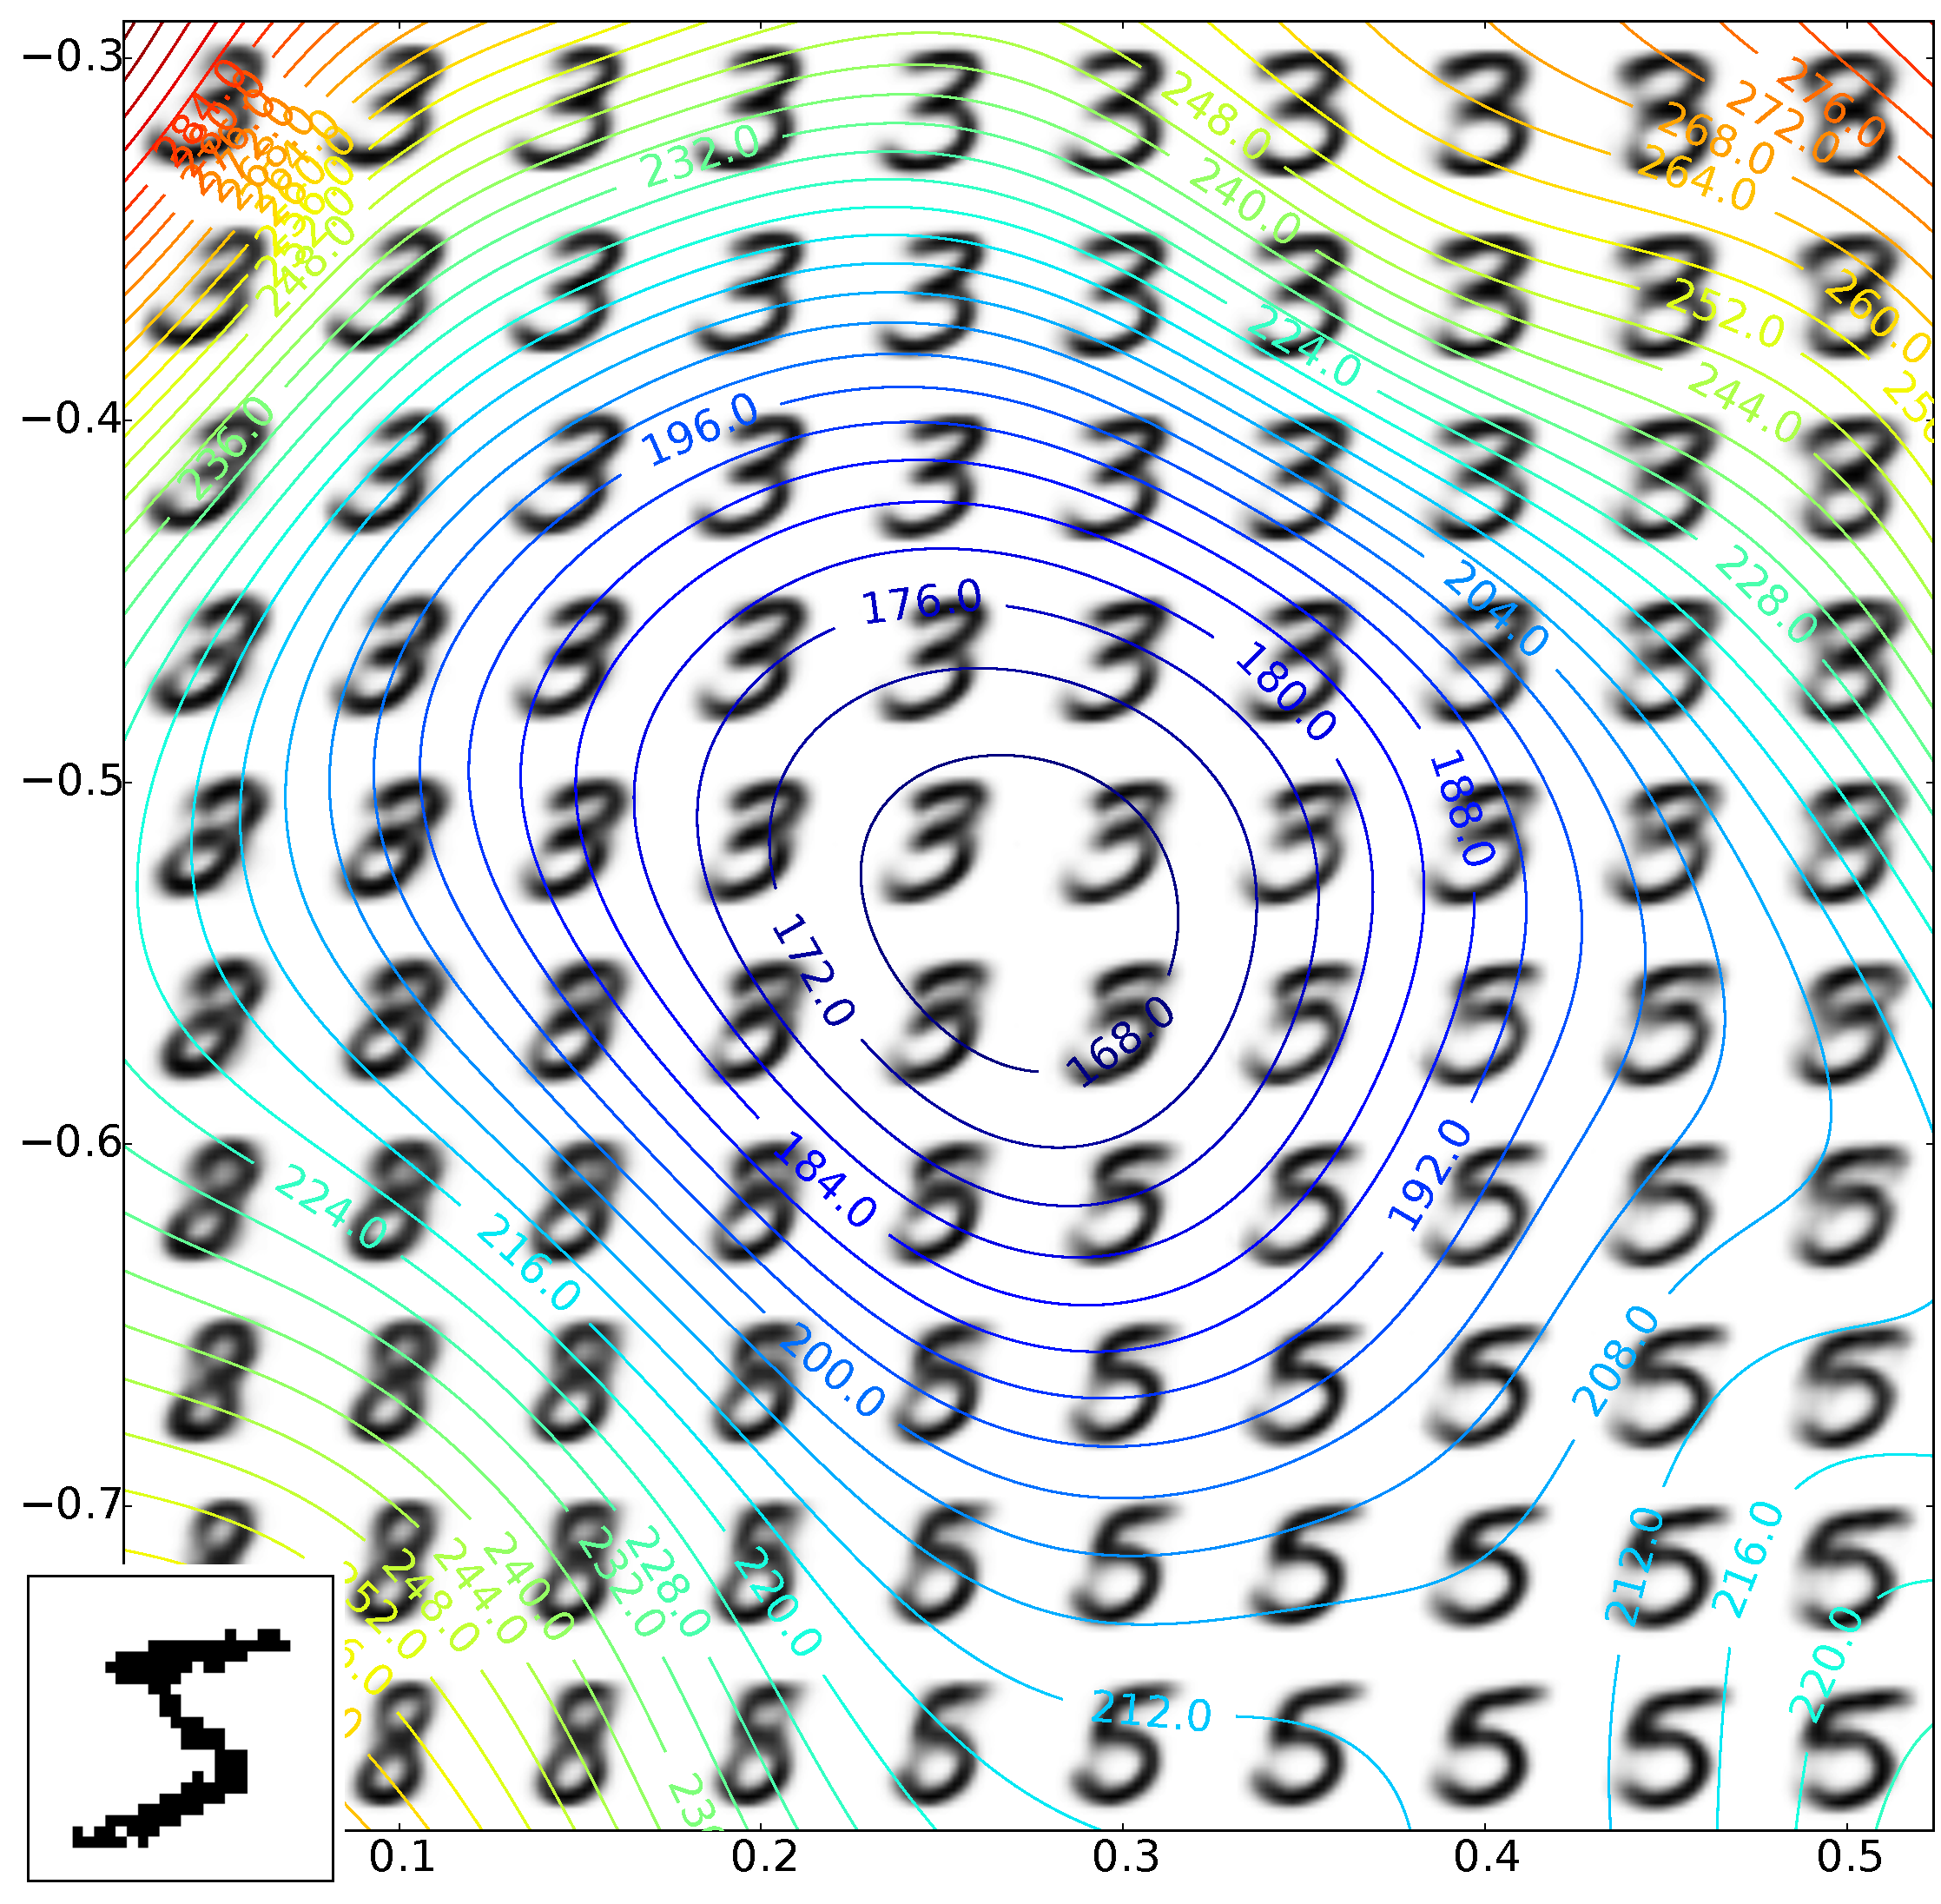
\includegraphics[width=\columnwidth]{figures/vae_pot_energy_example_with_inset.pdf}
\caption{Potential energy surface for the observed digit shown in the inset. The contours indicate the potential energy surface produced by a trained model with a 2-dimensional latent space. The plot also shows the mean images produced by the decoding model at evenly spaced points of the latent space.}
\label{fig:EnergySurfaceMNIST}
\end{figure}

\section{Visualizations of latent space}
\label{app:LatentVisualizations}

For each MNIST digit $x$ the potential energy surface given by $-\log p(x, z)$ differs. Figure~\ref{fig:EnergySurfaceMNIST} shows the energy surface produced by a trained model for a specific digit. For an intuitive understanding of the potential energy it also shows the mean images produced by the decoding model $p(x|z)$ at evenly spaced points in latent space. The closer the mean image is to the observed digit, the lower the potential energy.

For the best performing model on two-dimensional latent space figure~\ref{fig:2d_latent_visualization} illustrates the learnt latent space, depicting both exemplary mean images produced by the decoding model $p(x|z)$ and the latent space coordinates of the training set under the learnt encoder (including the HMC steps). A clear (but not perfect) separation of the digits is immediately obvious, showing the power of this unsupervised model to capture structures in the data. Interestingly, the latent space is not occupied evenly, with transition areas between the digits completely vacant. With a more flexible decoder this behaviour should become less prominent.

\begin{figure}[hb]
\centering
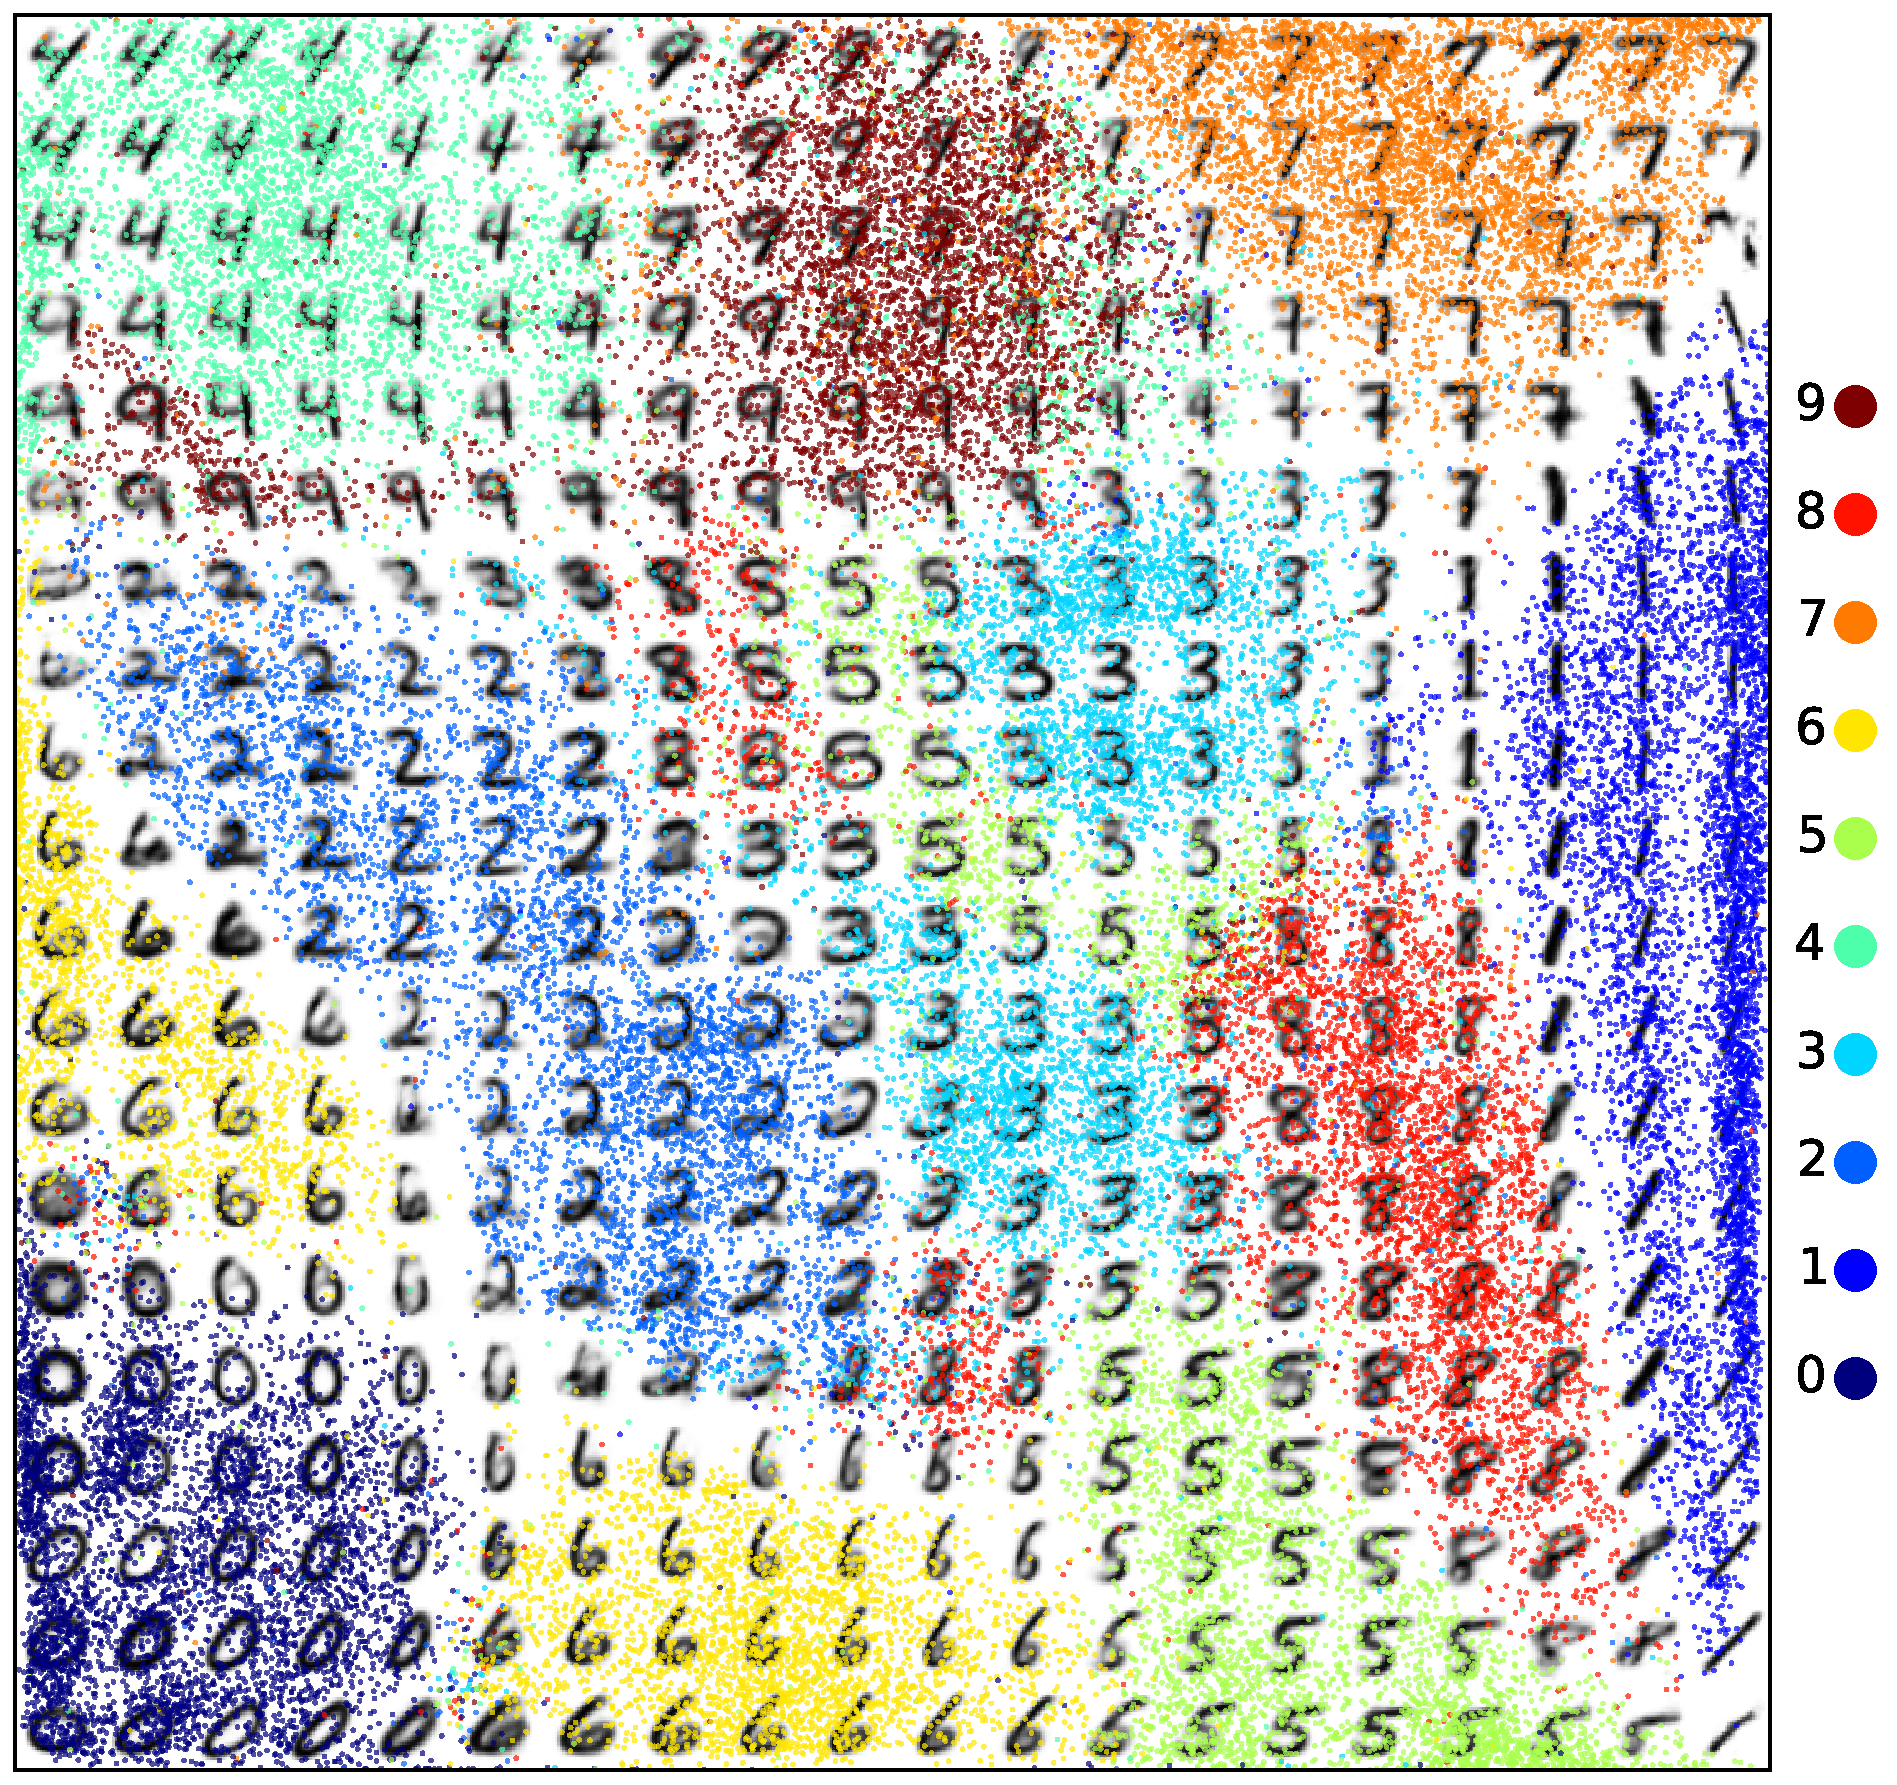
\includegraphics[width=\columnwidth]{figures/learned_representation_train_points_small.pdf}
\caption{Illustration of the two-dimensional latent space representation learnt by the model HMCVI 8 (see table~\ref{tab:Results}). To compensate for the Gaussian prior on the latent variables, linearly spaced coordinates in the unit square were transformed using the inverse Gaussian cdf. Therefore, the prior density in this view of latent space is uniform. For each coordinate the mean image produced by the decoder is shown. Additionally, the latent space representation of the training dataset as produced by the enhanced encoder is depicted (transformed by the Gaussian cdf), where each digit class is indicated by a different color.}
\label{fig:2d_latent_visualization}
\end{figure}

\end{appendices}
\end{document}

\end{document}